\chapter{Eksperymenty}
\label{chapter:eksperymenty}
% plan eksperymentow, opis danych, wyniki i wnioski
W niniejszym rozdziale przedstawione są eksperymenty, które zostały
przeprowadzone na zebranych wcześniej danych.
Opisany jest sposób ich wykonania, ich wyniki i wnioski, które z nich wynikają.
Na początku w sekcji \ref{section:opisdanych} opisana jest charakterystyka
zebranych danych, a następnie opisuję eksperymenty związane z analizą sentymentu
\ref{section:analizasentymentu2}, analizą społeczną 
\ref{section:analizaspoleczna} i analizą geolokacji 
\ref{section:analizageograficzna}.














%%%%%%%%%%%%%%%%%%%%%%%%%%%%%%%%%%%%%%%%%%%%%%%%%%%%%%%%%%%%%%%%%%% OPIS DANYCH
\section{Opis zebranych danych}
\label{section:opisdanych}
% 300 slow kluczowych, 18 druzyn, 50 meczow, daty,
% 7 mln tweetów, z tego 300 bylo retweetow, 800 z geolokacja, itd

Pomiędzy październikiem a grudniem 2013 roku zebrano 7 263 523 tweety związane
z piłką nożną. Pierwszy z nich ma datę 23 października 15:35:24 a ostatni
29 grudnia 19:27:27. Wszystkie wpisy są powiązane z rozegranymi w tym czasie
35 spotkaniami klubów Arsenal F.C. , Chelsea F.C., Manchester United F.C. i
Manchester City F.C. Daje to średnio 207 529 tweetów na mecz i niecałe
1 815 880 tweetów na drużynę.

Do zbierania tweetów użyte zostały dane 30 drużyn z 538 piłkarzami.
Dodając do tego popularne określenia menadżerów, piłkarzy czy klubów sumarycznie
zebrano 777 słów kluczowych, co daje średnio 22 słowa kluczowe na mecz.

Wpisy zostały stworzone przez 1 567 435 użytkowników, czyli 4.6 
wpisu na użytkownika. \mbox{222 545 wpisów} zawiera informacje o geolokacji, co 
stanowi zaledwie 3.06\% liczby wszystkich wpisów. \mbox{666 199 wpisów} to 
odpowiedzi (ang. \textit{replies}), to jest 9.17\%, natomiast aż 3 143 060 
tweetów jest retweetami pokrywając 43.27\% danych.

W tabeli \ref{table:listameczow} prezentuję listę wszystkich meczów, które były 
nasłuchiwane wraz z podstawowymi informacjami na ich temat.



\clearpage

\begin{table}[ht!]  
\begin{center}  
\begin{tabular}{|r|l|l|l|r|r|}
\hline
Lp. & Data & Gospodarz & Gość & Tweetów & Geolok.
\\ \hline 
1 & 2013-11-23 16:00 & Arsenal Londyn & Southampton FC & \texttt{190028} & \texttt{5231}	\\ \hline
2 & 2013-11-26 20:45 & FC Basel & Chelsea Londyn & \texttt{121209} & \texttt{3339}	\\ \hline
3 & 2013-11-26 20:45 & Arsenal Londyn & Olympique Marseille & \texttt{185252} & \texttt{6255}	\\ \hline
4 & 2013-11-27 20:45 & Manchester City & Viktoria Plzen & \texttt{24990} & \texttt{792}	\\ \hline
5 & 2013-11-27 20:45 & Bayer Leverkusen & Manchester United & \texttt{199232} & \texttt{6242}	\\ \hline
6 & 2013-11-30 16:00 & Cardiff City FC & Arsenal Londyn & \texttt{233151} & \texttt{6316}	\\ \hline
7 & 2013-12-01 13:00 & Tottenham Hotspur & Manchester United & \texttt{166394} & \texttt{4628}	\\ \hline
8 & 2013-12-01 17:10 & Chelsea Londyn & Southampton FC & \texttt{241768} & \texttt{7536}	\\ \hline
9 & 2013-12-01 17:10 & Manchester City & Swansea City & \texttt{29977} & \texttt{785}	\\ \hline
10 & 2013-12-04 20:45 & Sunderland AFC & Chelsea Londyn & \texttt{60047} & \texttt{1997}	\\ \hline
11 & 2013-12-04 20:45 & Manchester United & Everton FC & \texttt{182406} & \texttt{6226}	\\ \hline
12 & 2013-12-04 20:45 & Arsenal Londyn & Hull City & \texttt{200456} & \texttt{5076}	\\ \hline
13 & 2013-12-04 21:00 & West Bromwich Albion & Manchester City & \texttt{17783} & \texttt{608}	\\ \hline
14 & 2013-12-07 13:45 & Manchester United & Newcastle United & \texttt{416647} & \texttt{12613}	\\ \hline
15 & 2013-12-07 16:00 & Stoke City & Chelsea Londyn & \texttt{148780} & \texttt{4337}	\\ \hline
16 & 2013-12-07 16:00 & Southampton FC & Manchester City & \texttt{48101} & \texttt{1481}	\\ \hline
17 & 2013-12-08 17:00 & Arsenal Londyn & Everton FC & \texttt{381568} & \texttt{13057}	\\ \hline
18 & 2013-12-10 20:45 & Manchester United & Shakhtar Donetsk & \texttt{180301} & \texttt{6264}	\\ \hline
19 & 2013-12-10 20:45 & Bayern Monachium & Manchester City & \texttt{145381} & \texttt{4957}	\\ \hline
20 & 2013-12-11 20:45 & Chelsea Londyn & Steaua Bucuresti & \texttt{66125} & \texttt{1767}	\\ \hline
21 & 2013-12-11 20:45 & Napoli & Arsenal Londyn & \texttt{225461} & \texttt{7359}	\\ \hline
22 & 2013-12-14 13:45 & Manchester City & Arsenal Londyn & \texttt{525799} & \texttt{15561}	\\ \hline
23 & 2013-12-14 16:00 & Chelsea Londyn & Crystal Palace & \texttt{90541} & \texttt{2889}	\\ \hline
24 & 2013-12-15 14:30 & Aston Villa & Manchester United & \texttt{217221} & \texttt{6486}	\\ \hline
25 & 2013-12-21 16:00 & Manchester United & West Ham United & \texttt{171947} & \texttt{3975}	\\ \hline
26 & 2013-12-21 16:00 & Fulham FC & Manchester City & \texttt{63624} & \texttt{1624}	\\ \hline
27 & 2013-12-23 21:00 & Arsenal Londyn & Chelsea Londyn & \texttt{622011} & \texttt{19033}	\\ \hline
28 & 2013-12-26 13:45 & Hull City & Manchester United & \texttt{307313} & \texttt{8056}	\\ \hline
29 & 2013-12-26 16:00 & Chelsea Londyn & Swansea City & \texttt{109200} & \texttt{3264}	\\ \hline
30 & 2013-12-26 16:00 & West Ham United & Arsenal Londyn & \texttt{275811} & \texttt{8276}	\\ \hline
31 & 2013-12-26 18:30 & Manchester City & Liverpool FC & \texttt{331574} & \texttt{12009}	\\ \hline
32 & 2013-12-28 16:00 & Manchester City & Crystal Palace & \texttt{70251} & \texttt{2057}	\\ \hline
33 & 2013-12-28 16:00 & Norwich City & Manchester United & \texttt{204775} & \texttt{5348}	\\ \hline
34 & 2013-12-29 14:30 & Newcastle United & Arsenal Londyn & \texttt{339908} & \texttt{10624}	\\ \hline
35 & 2013-12-29 17:00 & Chelsea Londyn & Liverpool FC & \texttt{468494} & \texttt{16477}	\\ \hline
\end{tabular} 
\end{center} 
\caption{Lista meczów, które były nasłuchiwane}
\label{table:listameczow}
\end{table}





















%%%%%%%%%%%%%%%%%%%%%%%%%%%%%%%%%%%%%%%%%%%%%%%%%%%%%%%%%%%% PLAN EKSPERYMENTÓW
\section{Plan eksperymentów}
W ramach eksperymentów chcę udowodnić sensowność zastosowania zarówno
analizy sentymentu jak i geolokacji w analizie użytkowników sieci 
społecznościowych. Przedstawię serię badań pokazujących w jaki sposób
można zastosować te dwie dziedziny odkrywające nową wiedzę dotyczącą sieci
społecznych. Pokażę do czego można użyć sentymentu, do czego geolokacji
i w jaki sposób je połączyć.

Eksperymenty, które przedstawię to:
\begin{itemize}
  \item wartość sentymentu w kolejnych meczach 
  \ref{subsection:sentymentwmeczach},
  
  \item aktywność użytkowników i sentyment w ciągu meczu
  \ref{subsection:aktywnoscwmeczu},
  
  \item sposoby komunikacji między zwolennikami i przeciwnikami klubu 
  \ref{subsection:rodzajekomunikacji},
  
  \item sentyment wypowiedzi w relacjach między użytkownikami
  \ref{subsection:sentymentwrelacjach},
  
  \item struktura grup użytkowników w kolejnych meczach
  \ref{subsection:strukturagrup},
  
  \item odległość między użytkownikami a częstość kontaktów
  \ref{subsection:odlegloscmiedzyuzytkownikami},
  
  \item rozkład wpisów na mapie świata
  \ref{subsection:rozkladnamapie},
  
  \item odległość kibiców od miejsca rozgrywania meczu
  \ref{subsection:odlegloscodstadionu},
  
  \item rozkład wpisów z geolokacją
  \ref{subsection:geowpisy}.
\end{itemize}

W większości przypadków przedstawiam eksperymenty dla jednej, dwóch drużyn.
Jeśli nie zaznaczono inaczej, takie same prawidłowości zauważono dla
pozostałych zespołów.






% %%%%%%%%%%%%%%%%%%%%%%%%%%%%%%%%%%%%%%%%%%%%%%%%%%%%%%%%%%% ANALIZA SENTYMENTU
\section{Analiza sentymentu}
\label{section:analizasentymentu2}
% 40\% bylo pozytywnych, 30\% negatywnych w meczach Arsenalu byl taki a taki sentyment

Analiza sentymentu została przeprowadzona zgodnie z algorytmem przedstawionym w
rozdziale \ref{section:analizasentymentu}. W związku z tym, że wpisy typu
retweet nie mogą posiadać sentymentu wszystkie zaprezentowane poniżej analizy
odnoszą się do grupy wpisów nie będących retweetami. To daje nam 4 120 463
tweety, nad którymi były prowadzone badania. W tej grupie 2 005 934 wpisy
zostały oznaczone jako pozytywne -- 48.68\%, a 1 944 448 jako negatywne --
47,19\%.



\subsection{Sentyment w meczach}
\label{subsection:sentymentwmeczach}
Pierwszym eksperymentem jaki został przeprowadzony było zbadanie tego w jaki 
sposób zmienia się wydźwięk wypowiedzi pomiędzy kolejnymi meczami danej drużyny.
W tym celu zbadany został ogólny sentyment podczas danego wydarzenia sportowego.
Na wykresach \ref{image:pozytywnosc-arsenal} oraz 
\ref{image:pozytywnosc-munited} przedstawione są wyniki tych badań.
Wartość pozytywności została wyliczone zgodnie z opisem z sekcji
\ref{subsection:ocenapozytywnosci}.

\clearpage

\begin{figure}[ht!]
\centering
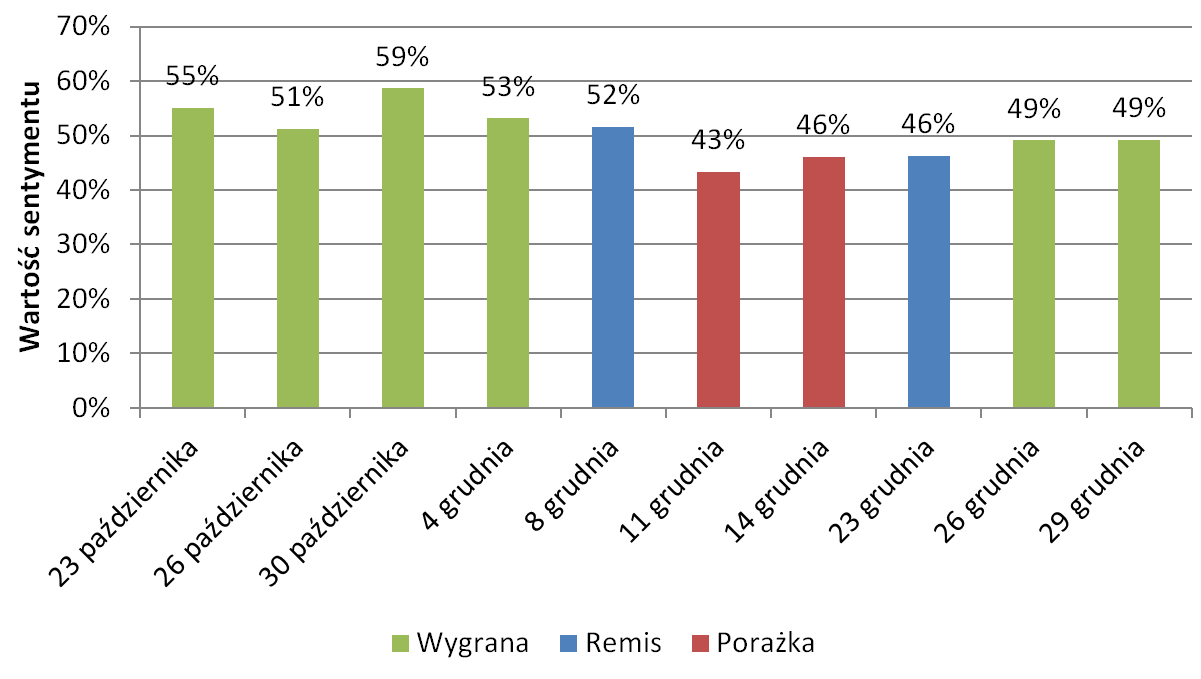
\includegraphics[width=120mm]{img/pozytywnosc-arsenal2.png}
\caption{Wyniki spotkań Arsenalu a sentyment wpisów}
\label{image:pozytywnosc-arsenal}
\end{figure}

\begin{figure}[ht!]
\centering
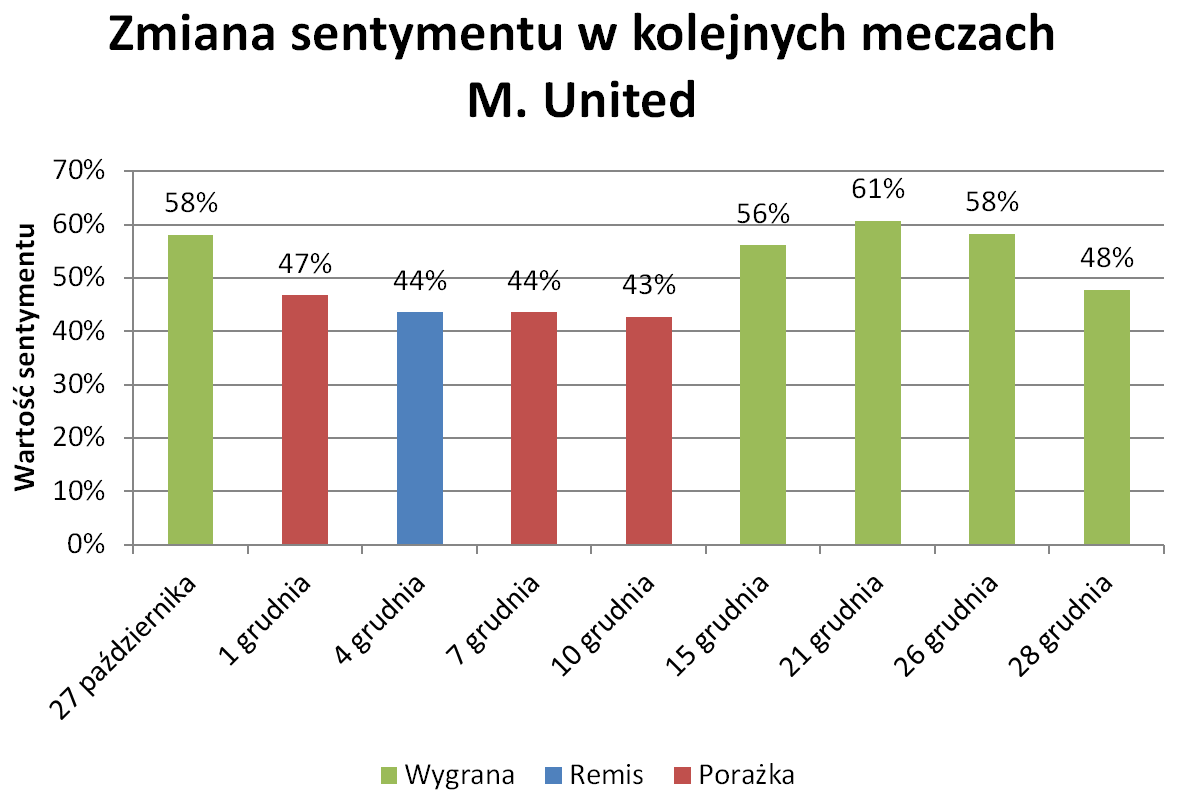
\includegraphics[width=120mm]{img/pozytywnosc-munited2.png}
\caption{Wyniki spotkań Manchesteru United a sentyment wpisów}
\label{image:pozytywnosc-munited}
\end{figure}

\subsubsection{Obserwacje i wnioski}
Posiadając informację na temat końcowego wyniku danego meczu łatwo można 
zauważyć, iż wartość sentymentu jest adekwatna do uzyskanego rezultatu danej 
drużyny. Gdy Arsenal odnosi zwycięstwo wówczas wpisy mają częściej wydźwięk
pozytywny przekraczając w większości przypadków wartość 50\%. Gdy jednak 
drużyna przegrywa nacechowanie emocjonalne wpisów wyraźnie spada poniżej 46\%.
Również mecz zakończony remisem powoduje raczej wpisy niezadowolenia.
 
Tę samą prawidłowość można zauważyć analizując wyniki badań dla meczów
Manchesteru United. Gdy drużyna wygrywa, wówczas zadowolenia we wpisach sięga
nawet 61\%, a gdy ponosi porażkę -- wynik sentymentu spada do czterdziestu kilku
procent.

Po analizie tych badań nasuwają się oczywiste wnioski. Sposób reagowania
internautów na wyniki ich drużyn jest dokładnie taki sam jak rezultat przez nie
osiągany. Gdy drużyna wygrywa, okazuje się lepsza, to tak samo jak w życiu, jej
kibice wykazują radość, szczęście, zadowolenie i inne pozytywne emocje.
Natomiast gdy klub przegrywa mecz, wówczas wśród tweetów dużo łatwiej o wpisy o
nacechowaniu negatywnym. Widać więc, że reakcje użytkowników Twittera są
dokładnie takie same jak zwykłych kibiców -- odzwierciedlają ich aktualny stan
ducha po meczu ulubionej drużyny. Nie ma tutaj żadnej różnicy między światem
realnym a wirtualnym.















\subsection{Liczba tweetów i rozkład sentymentu w ciągu meczu}
\label{subsection:aktywnoscwmeczu}
Kolejny eksperyment jaki można wykonać na zgromadzonych danych
to zbadanie aktywności użytkowników Twittera w związku z wydarzeniami 
na boisku. Badanie takie można przeprowadzić dla każdego meczu, który znalazł 
się pośrod tych, które zostały pobrane. Poniżej przedstawione są rezultaty
dla spotkania pomiędzy drużynami Chelsea F.C. a Southampton F.C. (01.12.2013 r.),
które zakończyło się wynikiem 3-1. Są to dwa wykresy: pierwszy z liczbą tweetów
na minutę (z uwzględnieniem wyrażanego przez nie sentymentu) 
\ref{image:tweety-w-meczu} oraz drugi pokazujący zmianę sentymentu w trakcie
spotkania \ref{image:sentyment-w-meczu}.

Na obu wykresach zaznaczone są kluczowe wydarzenia:

\begin{enumerate}
  \item \textbf{17:10} -- 1 min., początek meczu i gol J. Rodriguez (Southampton FC) 0-1.
  \item \textbf{17:59} -- 45 + 4 min., koniec pierwszej połowy.
  \item \textbf{18:14} -- 45 min., początek drugiej połowy.
  \item \textbf{18:24} -- 55 min., gol G. Cahill (Chelsea FC) 1-1.
  \item \textbf{18:31} -- 62 min., gol J. Terry (Chelsea FC) 2-1.
  \item \textbf{18:59} -- 90 min., gol D. Ba (Chelsea FC) 3-1.
  \item \textbf{19:05} -- 90 + 6 min., koniec spotkania.
\end{enumerate}



\begin{figure}[ht!]
\centering
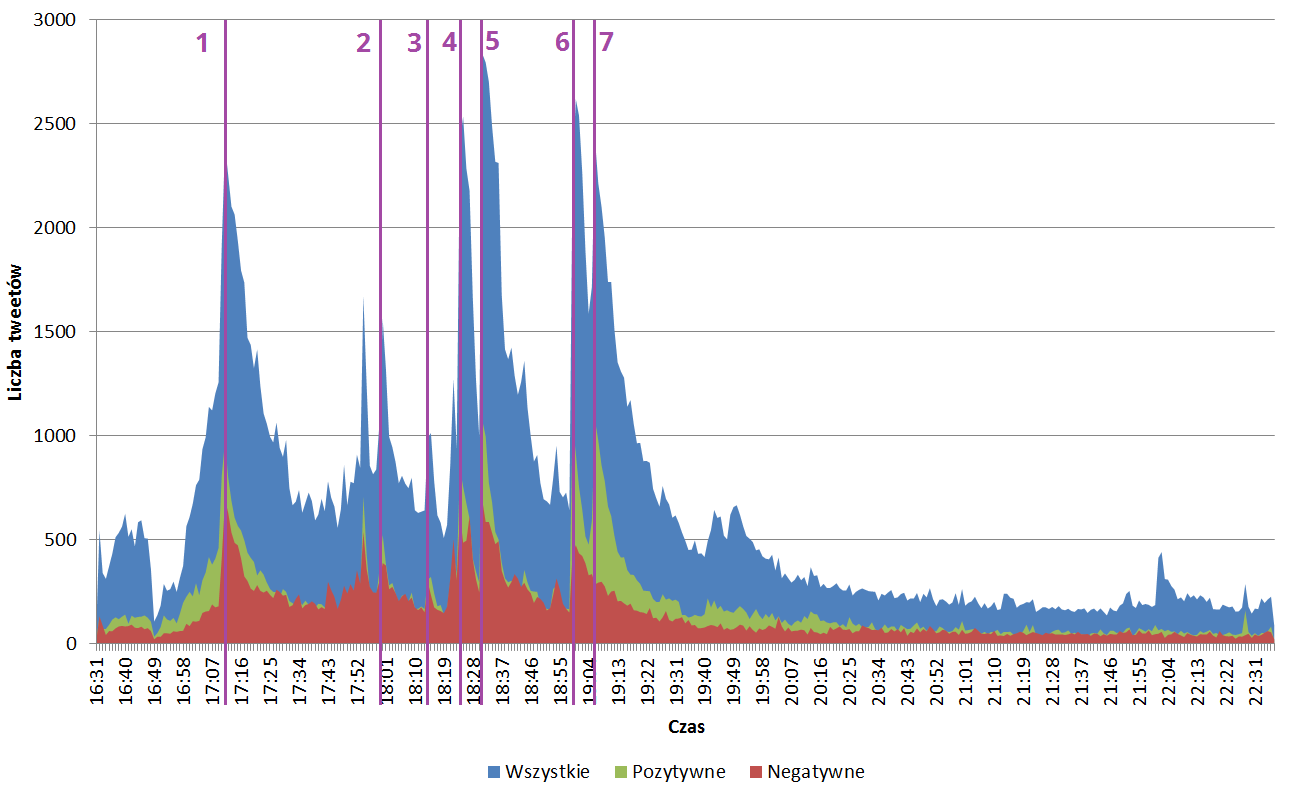
\includegraphics[width=160mm]{img/tweety-w-meczu-nums.png}
\caption{Zmiana liczby tweetów w trakcie meczu Chelsea -- Southampton}
\label{image:tweety-w-meczu}
\end{figure}

\begin{figure}[ht!]
\centering
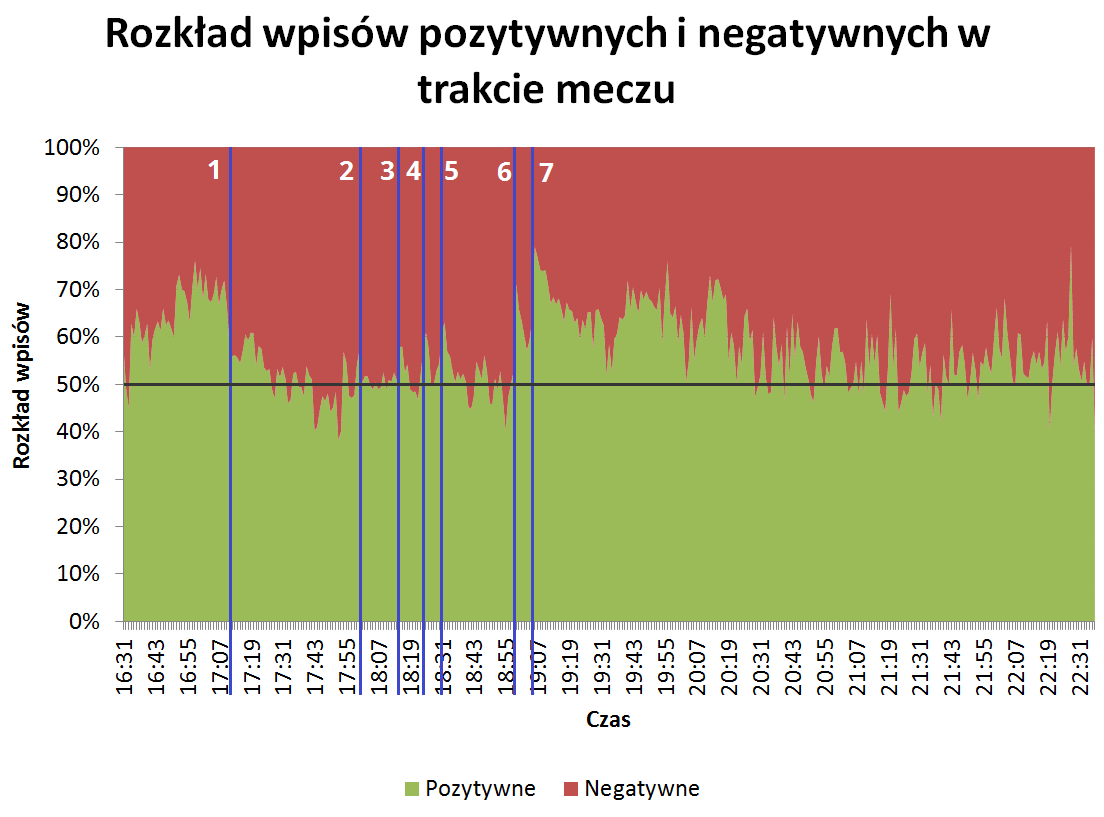
\includegraphics[width=140mm]{img/sentyment-w-meczu-nums-50percentage.png}
\caption{Rozkład sentymentu tweetów w trakcie meczu Chelsea -- Southampton}
\label{image:sentyment-w-meczu}
\end{figure}


\subsubsection{Obserwacje i wnioski}
Na pierwszym załączonym wykresie wyraźnie widać silną korelację istotnych
wydarzeń boiskowych z wysokim wzrostem liczby wysyłanych tweetów. 
Liczba ta rośnie nawet trzykrotnie w przypadku strzelonej bramki przez jedną
z drużyn. Użytkownicy Twittera dużo mocniej angażują się w komentowanie i 
komunikację poprzez to medium w najważniejszych momentach danego spotkania.
Można zauważyć, że początek i koniec spotkania są momentami, w których
kibice generują stosunkowo dużą liczbę wpisów. W trakcie spotkania
ich aktywność wzrasta, gdy na boisku dzieje się coś ciekawego.
Po zakończonym meczu liczba wpisów stopniowo maleje, a dane spotkanie
nie cieszy się już zainteresowaniem takiego szerokiego grona
odbiorców jak wcześniej. Są to już zapewne raczej wiadomości wysyłane
przez bardziej zagorzałych fanów, analizujących dane spotkanie dłużej,
wyciągających z niego wnioski, a nie tych osób, które były zainteresowane
meczem tylko wtedy gdy ten się jeszcze odbywał.

Drugi wykres przedstawiający zmiany sentymentu wyraźnie pokazuje, że wpisy były
wyrównane w trakcie meczu (jeśli chodzi o proporcje sentymentu), aż do momentu,
w którym Chelsea FC zdobyła bramkę na 3-1, ustalając w ten sposób de facto
końcowy wynik spotkania. Wówczas wyraźnie przeważały wpisy o wydźwięku
pozytywnym. Sam fakt tego, że to właśnie te tweety były liczniejsze może wynikać
między innymi z tego, że Chelsea to klub mający więcej fanów na całym świecie
niż Southampton, grający w ostatnich latach regularnie w Lidze Mistrzów, bijący
się o zwycięsto w Premier League, czy jeżdżący w trakcie przygotowań do sezonu
na tournee do Stanów Zjednoczonych i Azji. Southampton natomiast to klub z dolnej
części tabeli, mający zupełnie inne cele w trakcie sezonu, nieposiadający tyle
gwiazd, w związku z czym nie skupiający wokół siebie takiego zainteresowania.

Bardzo podobne wykresy można uzyskać analizując także inne spotkania.
Tam również internauci mocniej angażują się, gdy dzieje się coś ciekawego, a
sentyment jest zgodny z wynikiem i liczbą przeważających kibiców danego klubu.
Widać więc, że Twitter jest miejscem, w którym jego użytkownicy uzewnętrzniają
swoje emocje błyskawicznie, gdy dzieje się coś co ich porusza.
Są to takie same naturalne emocje, których doświadczają oni na co dzień, nie są
w żaden sposób wyimaginowane, przemyślane, czy sterowane, ale pokazują aktualny
stan ducha danej społeczności. Można więc dojść do wniosku, że badanie Twittera
może przynieść nam wyniki, do których powinniśmy podejść poważnie i nie
bagatelizować ich twierdząc, że być może w internecie osoby zachowują się
inaczej niż w codziennym życiu.




%%%%%%%%%%%%%%%%%%%%%%%%%%%%%%%%%%%%%%%%%%%%%%%%%%%%%%%%%%%%%% ANALIZA SPOŁECZNA

\section{Analiza sieci społecznych}
\label{section:analizaspoleczna}
Do analizy sieci społecznych zostały użyte dane użytkowników pobrane 
równocześnie ze ściąganiem wpisów. Relacje między użytkownikami zostały
zbudowane na podstawie informacji zawartych w tweetach. Są to więc
dwa rodzaje relacji -- odpowiedzi i retweety. Z ich pomocą przeprowadzone
zostały badania nad siecią społeczną, którą tworzą użytkownicy Twittera. 






\subsection{Liczba i rodzaje komunikacji między zwolennikami i przeciwnikami klubów}
\label{subsection:rodzajekomunikacji}
% retweety pozytywne zwolennicy, replies negatywne, przeciwnicy, itd

Jednym z eksperymentów przeprowadzonych w analizie sieci społecznych było
sprawdzenie rodzaju komunikacji pomiędzy użytkownikami. 
Dodatkowo użytkownicy zostali podzieleni na zwolenników i przeciwników danego 
klubu zgodnie z opisem w sekcji \ref{subsubsection:wykrywaniezwolennikow}.


\subsubsection{Charakterystyka komunikacji poprzez odpowiedzi (\textit{replies})}
Zbadana został sposób w jaki komunikują się użytkownicy Twittera korzystając
z funkcji \textit{odpowiedz}, polegającej na możliwości komentowania wpisów
innych użytkowników. Tak jak było to wcześniej zaznaczone w tym serwisie
społecznościowym użytkownicy do woli mogą komentować wpisy osób, których
nie mają na swoich listach znajomych.

Poprzez podzielenie użytkowników na grupy zwolenników i przeciwników -- na
przykładzie wpisów dotyczących Manchesteru United -- można zauważyć ciekawe
obserwacje. Wykres przedstawiający wyniki badań przedstawia rysunek 
\ref{image:replies-munited}.

\begin{figure}[ht!]
\centering
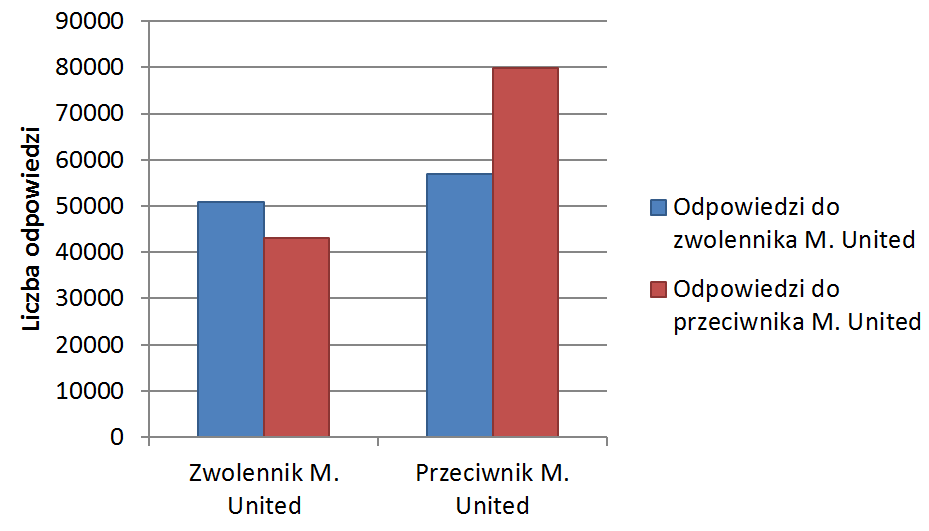
\includegraphics[width=120mm]{img/replies-munited.png}
\caption{Charakterystyka odpowiedzi wśród wpisów dotyczących Manchesteru United}
\label{image:replies-munited}
\end{figure}

\subsubsection{Obserwacje i wnioski}
Wykres przedstawia liczbę odpowiedzi zwolenników i przeciwników Manchesteru 
United na wpisy zwolenników i przeciwników tego klubu. Na jego podstawie można
zauważyć, że na wpisy zwolenników częściej odpowiadają zwolennicy. 
Oznacza to, że ta grupa użytkowników trzyma się blisko siebie i osoby, które
są sympatykami Manchesteru również obserwują i komunikują się z innymi 
sympatykami tego klubu produkując większą liczbę wpisów.
Podobna zależność ma miejsce wśród przeciwników Manchesteru United.
Wpis przeciwnika tego klubu bardziej angażuje do dyskusji również innych
przeciwników. Prawdopodobnie osoby biorące udział w tej dyskusji wspólnie
narzekają na grę tego zespołu, wzajemnie nakręcając się do ożywionych dyskusji.

Na podstawie powyższego wykresu widać więc, że użytkownicy Twittera lubią 
tworzyć grupy o podobnych zainteresowaniach czy sympatiach. Dany użytkownik
częściej będzie komunikował się z osobami, które myślą podobnie jak on,
umacniając w ten sposób swoje przekonanie o własnych przemyśleniach na dany temat.
Gdy ktoś jest zwolennikiem danego klubu częściej dyskutuje z podobnymi sobie
internautami. Tak samo przeciwnicy łatwiej znajdują nić porozumienia między sobą
mając takie samo zdanie dotyczące określonego wydarzenia. Internauci lepiej
odnajdują się wśród osób podzielających ich opinie.  









\subsubsection{Charakterystyka komunikacji poprzez retweety}
Podobnie jak powyższe badanie został przeprowadzony eksperyment na temat 
charakterystyki komunikacji między użytkownikami korzystający z opcji 
\textit{retweet}. Polega ona na podaniu dalej wpisu, który uważamy za ciekawy.
Wyniki, które w ten sposób uzyskano różnią się od poprzednich i zaprezentowane
są na rysunku \ref{image:retweety-munited}.

\begin{figure}[ht!]
\centering
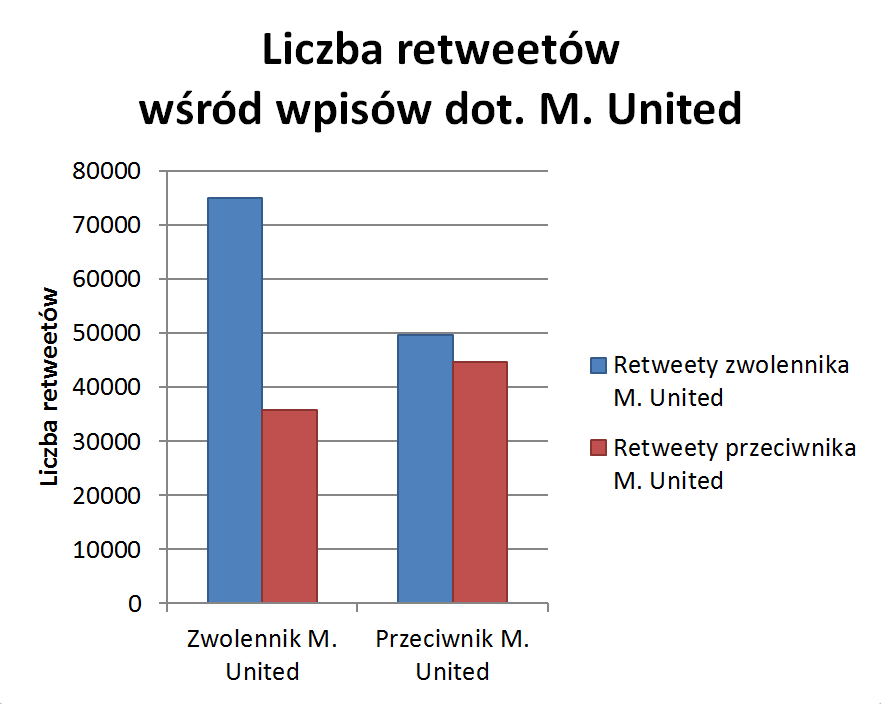
\includegraphics[width=120mm]{img/retweety-munited.png}
\caption{Charakterystyka retweetów wśród wpisów dotyczących Manchesteru United}
\label{image:retweety-munited}
\end{figure}



\subsubsection{Obserwacje i wnioski}
Tym razem widać zupełnie inne ułożenie słupków na wykresie.
Na pierwszy plan wyraźnie wysuwa się słupek pierwszy z lewej, który oznacza
liczbę wpisów zwolenników podanych dalej przez innych zwolenników. Widać więc,
że sympatycy Manchesteru United bardzo chętnie przekazują dalej wpisy 
pozostałych sympatyków. Mogą to być na przykład wpisy o strzelonym golu,
czy jakieś pozytywne opinie na temat danej drużyny. Najrzadziej z całej
czwórki zaprezentowanych relacji dochodzi do sytuacji, gdy przeciwnik
Manchseteru podaje dalej wpis zwolennika. Jeśli chodzi o retweetowanie
tweetów przeciwników Manchesteru United, to dochodzi do tego mniej więcej po
równo między przeciwnikami i zwolennikami.

Po analizie dwóch powyższych eksperymentów nasuwają się następujące wnioski.
Użytkownicy lubią gromadzić się w grupy o podobnych zainteresowaniach,
wspólnie komentując wydarzenia w podobny sposób. Zwolennicy i przeciwnicy
danego klubu zachowują się w charakterystyczny sposób. Ci pierwsi bardzo często
retweetują wpisy innych zwolenników, a ci drudzy częściej dyskutują ze sobą.





\subsection{Sentyment odpowiedzi między zwolennikami i przeciwnikami drużyny}
\label{subsection:sentymentwrelacjach}
Oprócz zbadania rodzaju i charakterystyki komunikacji pomiędzy użytkownikami 
Twittera przyjrzano się także bliżej komunikacji związanej z odpowiedziami 
(\textit{replies}). Przeprowadzono eksperyment, w którym zwrócono uwagę
na wydźwięk wpisów będących odpowiedziami na inne wpisy -- ponownie z podziałem
na zwolenników i przeciwników danej drużyny. W tej sekcji skupiam się tylko na
odpowiedziach, gdyż niemożliwe jest badanie sentymentu retweetów, które są
tylko podaniem dalej innych wpisów. Poniżej prezentuję jak rozkładał się
sentyment wpisów dla wszystkich kombinacji zwolenników i przeciwników
Arsenalu jako autorów i odpowiadających.


\subsubsection{Gdy odpowiada zwolennik Arsenalu}
Poniżej prezentuję dwie sytuacje, w których odpowiadającym na wpis jest
użytkownik będący zwolennikiem drużyny Arsenalu Londyn. W pierwszym przypadku
\ref{image:reply-sentiment-zwolennik-zwolennik} pokazana jest struktura
odpowiedzi zwolennika na wpisy innego zwolennika, zaś w drugim
\ref{image:reply-sentiment-zwolennik-przeciwnik} odpowiedzi odnoszą się do
wpisów przeciwnika klubu.

\begin{figure}[ht!]
\centering
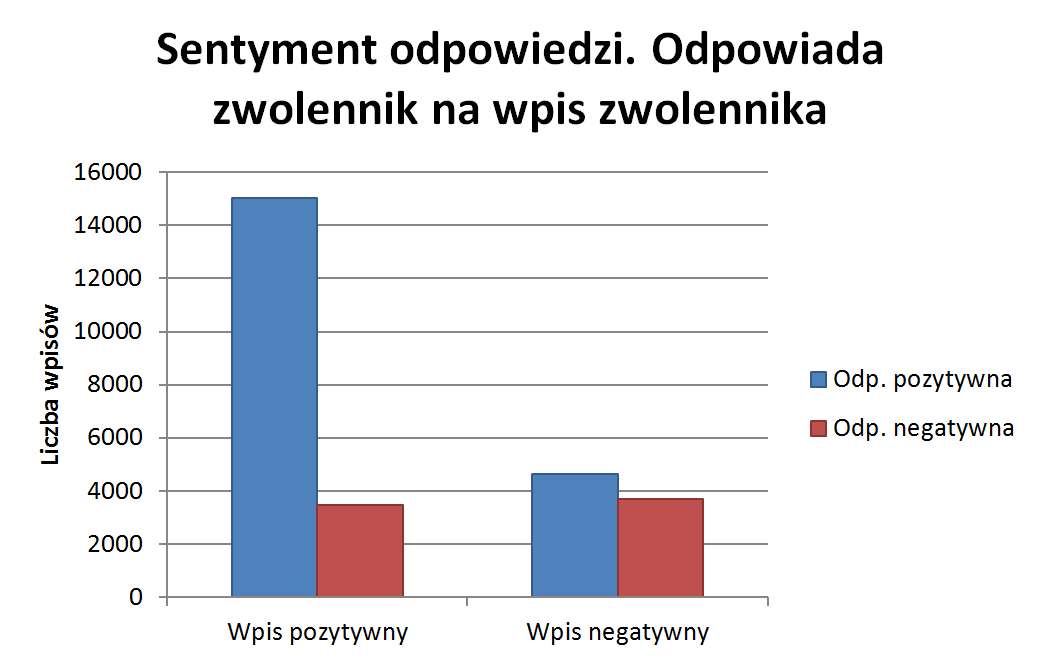
\includegraphics[width=120mm]{img/reply-sentiment-zwolennik-zwolennik.png}
\caption{Sentyment odpowiedzi. Odpowiada zwolennik Arsenalu na wpis zwolennika}
\label{image:reply-sentiment-zwolennik-zwolennik}
\end{figure}


\begin{figure}[ht!]
\centering
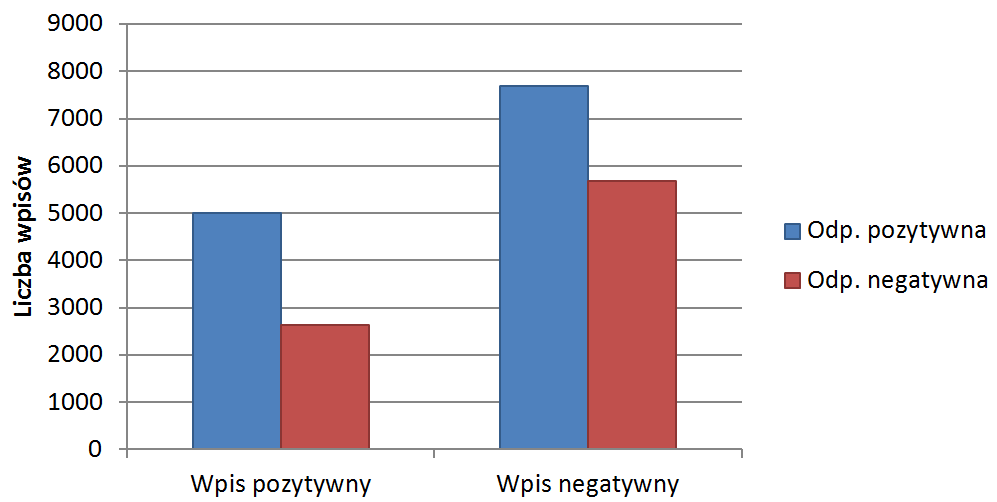
\includegraphics[width=120mm]{img/reply-sentiment-zwolennik-przeciwnik.png}
\caption{Sentyment odpowiedzi. Odpowiada zwolennik Arsenalu na wpis przeciwnika}
\label{image:reply-sentiment-zwolennik-przeciwnik}
\end{figure}



\subsubsection{Obserwacje i wnioski}
To co rzuca się na pierwszy rzut oka na zamieszczone wykresy to fakt, że 
zwolennicy danego klubu najczęściej tworzą wpisy pozytywne. Zauważalne jest to,
że wśród zwolenników dominującym modelem komunikacji jest wymiana wiadomości
o nacechowaniu pozytywnym -- na wpis pozytywny, odpowiedzą jest również wpis o 
takim samym sentymencie -- wyraźnie wyróżniająca się spośród pozostałych
wariantów.
Zauważyć można również to, że przeciwnicy Arsenalu generują więcej wpisów 
negatywnych, a mimo to sympatycy klubu z Londynu starają się im odpowiadać
tweetami o wydźwięku pozytywnym.

Widać więc, że osoby tworzące pozytywne wpisy na dany temat pobudzają się
wzajemnie do ożywionej dyskusji, a także starają się dbać o dobre imię
i dobry odbiór tematu, który jest im bliski. Tworzą więc grupę, która
dobrze czuje się w swoim towarzystwie, a także stara się kreować
pozytywny odbiór swojego ulubionego klubu na zewnątrz, wśród innych osób.

\subsubsection{Gdy odpowiada przeciwnik Arsenalu}
Analogicznie do poprzednich eksperymentów w dwóch wykresach poniżej (na 
rysunkach \ref{image:reply-sentiment-przeciwnik-zwolennik} i 
\ref{image:reply-sentiment-przeciwnik-przeciwnik}) zaprezentowane są
wyniki badań nad odpowiedziami przeciwnika Arsenalu na wpisy zwolenników
i przeciwników tego klubu.

\begin{figure}[ht!] \centering
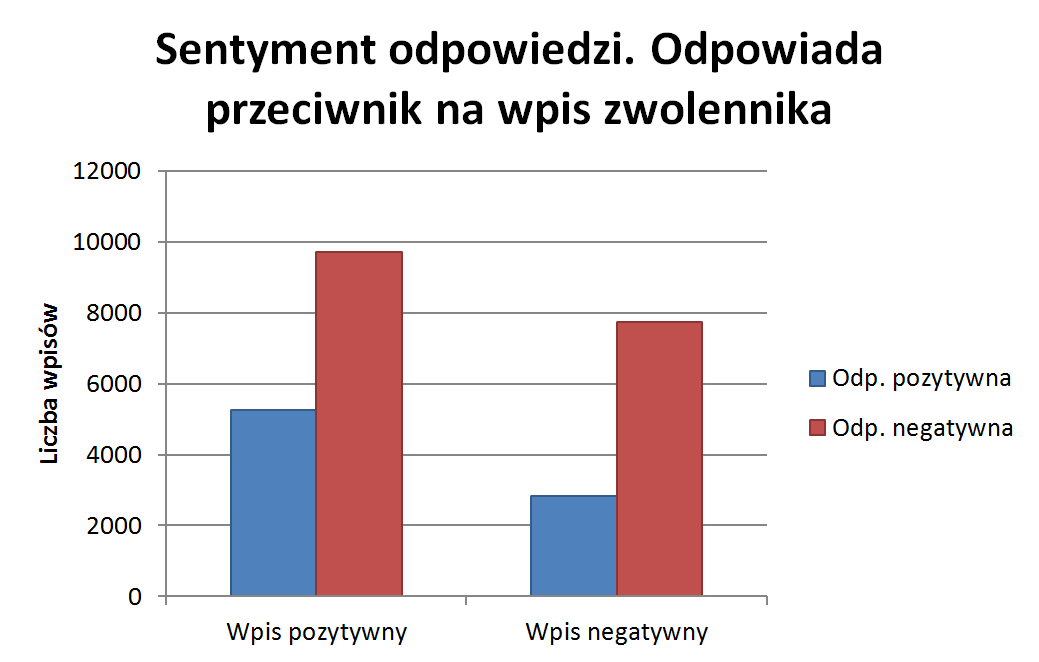
\includegraphics[width=120mm]{img/reply-sentiment-przeciwnik-zwolennik.png}
\caption{Sentyment odpowiedzi. Odpowiada przeciwnik Arsenalu na wpis zwolennika}
\label{image:reply-sentiment-przeciwnik-zwolennik}
\end{figure}

\clearpage
\begin{figure}[ht!] \centering
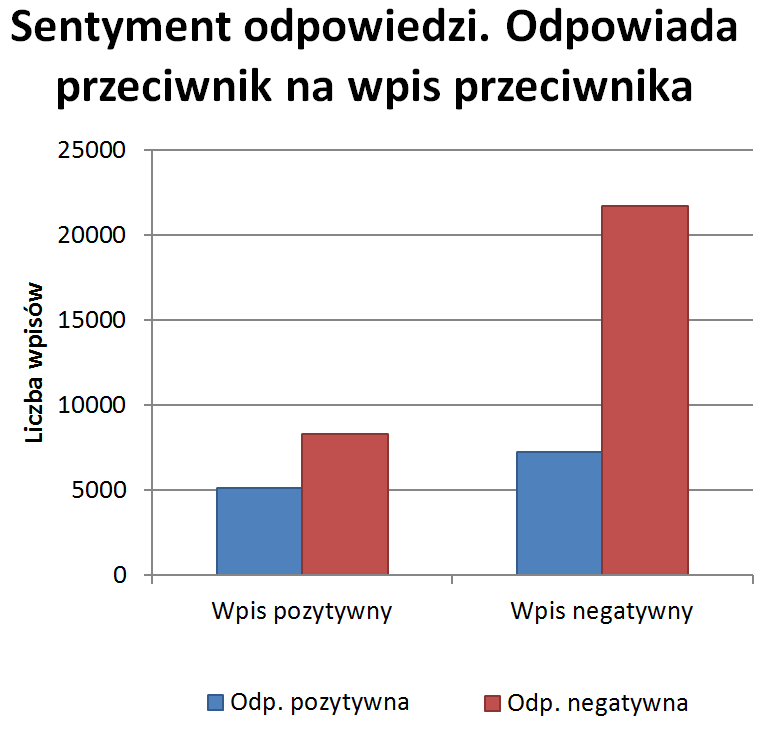
\includegraphics[width=120mm]{img/reply-sentiment-przeciwnik-przeciwnik.png}
\caption{Sentyment odpowiedzi. Odpowiada przeciwnik Arsenalu na wpis przeciwnika}
\label{image:reply-sentiment-przeciwnik-przeciwnik}
\end{figure}

\subsubsection{Obserwacje i wnioski}
Z powyższych wykresów można wywnioskować, że wpisy przeciwników mają najczęściej
wydźwięk negatywny. Gdy przeciwnik odpowiada na pozytywny wpis zwolennika, to tylko
1 na 3 wpisy są również pozytywne. Zdecydowanie częściej przeciwnik odpisuje
zwolennikowi wpisem o sentymencie negatywnym. 
Co warte zauważenia najwięcej odpowiedzi przeciwnicy Arsenalu wysyłają
pod wpisami negatywnymi innych przeciwników, również nacechowując swoje opinie
negatywnie.

Analogicznie więc jak w poprzednim eksperymencie widać, że przeciwnicy
Arsenalu tworzą wspólną grupę, w której wymieniają się swoimi
krytycznymi opiniami na temat tej drużyny. I tak samo jak poprzednio
wychodzą również z tymi opiniami do innych internautów, starając się
przekonać ich do swojego punktu widzenia.
















%%%%%%%%%%%%%%%%%%%%%%%%%%%%%%%%%%%%%%%%%%% ANALIZA GRUP W SIECIACH SPOŁECZNYCH
\subsection{Analiza grup w sieciach społecznych}
\label{subsection:strukturagrup}
Oprócz powyższych badań nad sposobami komunikacji i relacji budowanymi między
użytkownikami przeprowadzona została także analiza grup użytkowników 
pomiędzy meczami. Grupy te były budowane zgodnie z
opisem w sekcji \ref{subsubsection:koncepcja-wykrywaniegrup}.

Liczności tych grup zostało zaprezentowane na poniższych
wykresach pokazując jak zmieniały się z meczu na mecz.
Na pierwszym \ref{image:grupy-arsenal} przedstawione są dane
dla Arsenalu, a na drugim \ref{image:grupy-munited} dla Manchesteru United.
Oprócz wielkości poszczególnych grup wykresy prezentują także podobieństwo
zbioru użytkowników komentującego następujące po sobie wydarzenia.
Sposób wykrywania grup został opisany w sekcji
\ref{section:koncepcja-wykrywaniegrup} a sposób badania podobieństwa w sekcji
\ref{subsection:badaniepodobienstwagrup}.
 
\begin{figure}[ht!]
\centering
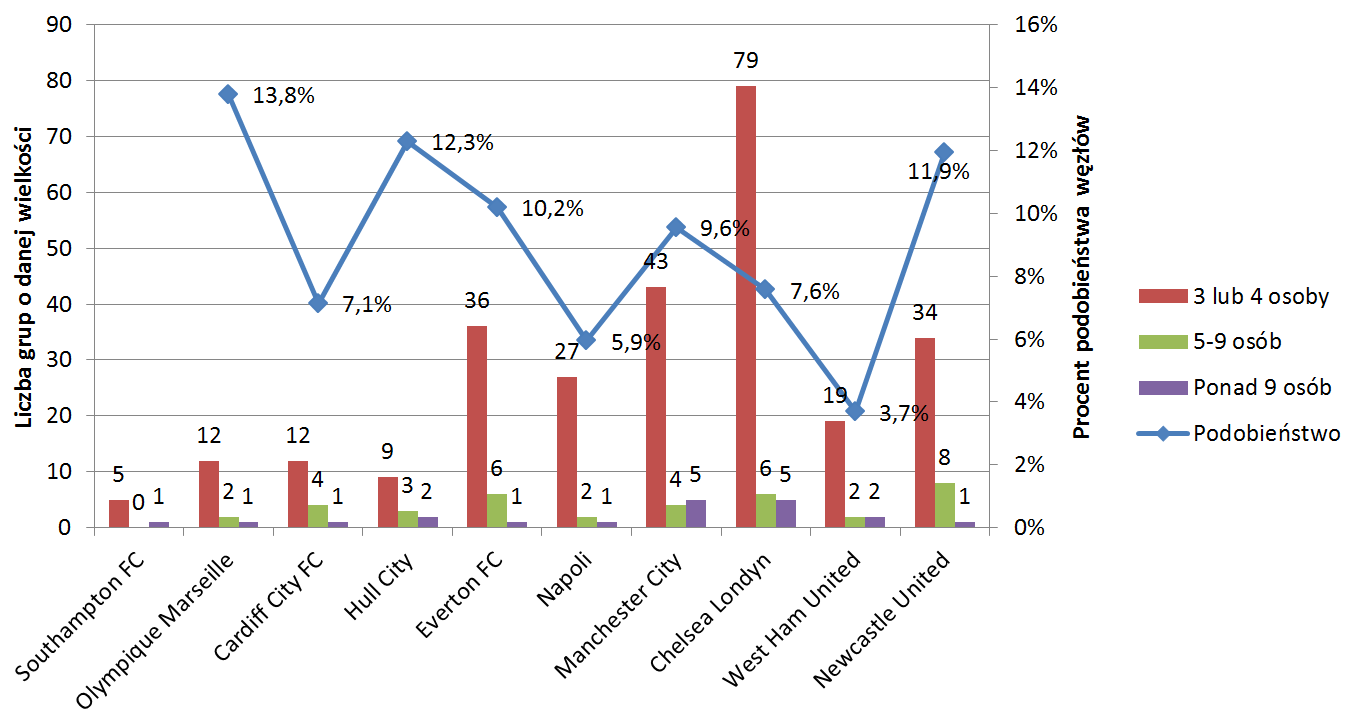
\includegraphics[width=160mm]{img/grupy-arsenal-nums.png}
\caption{Struktura grup użytkowników w meczach Arsenalu}
\label{image:grupy-arsenal}
\end{figure}

\begin{figure}[ht!]
\centering
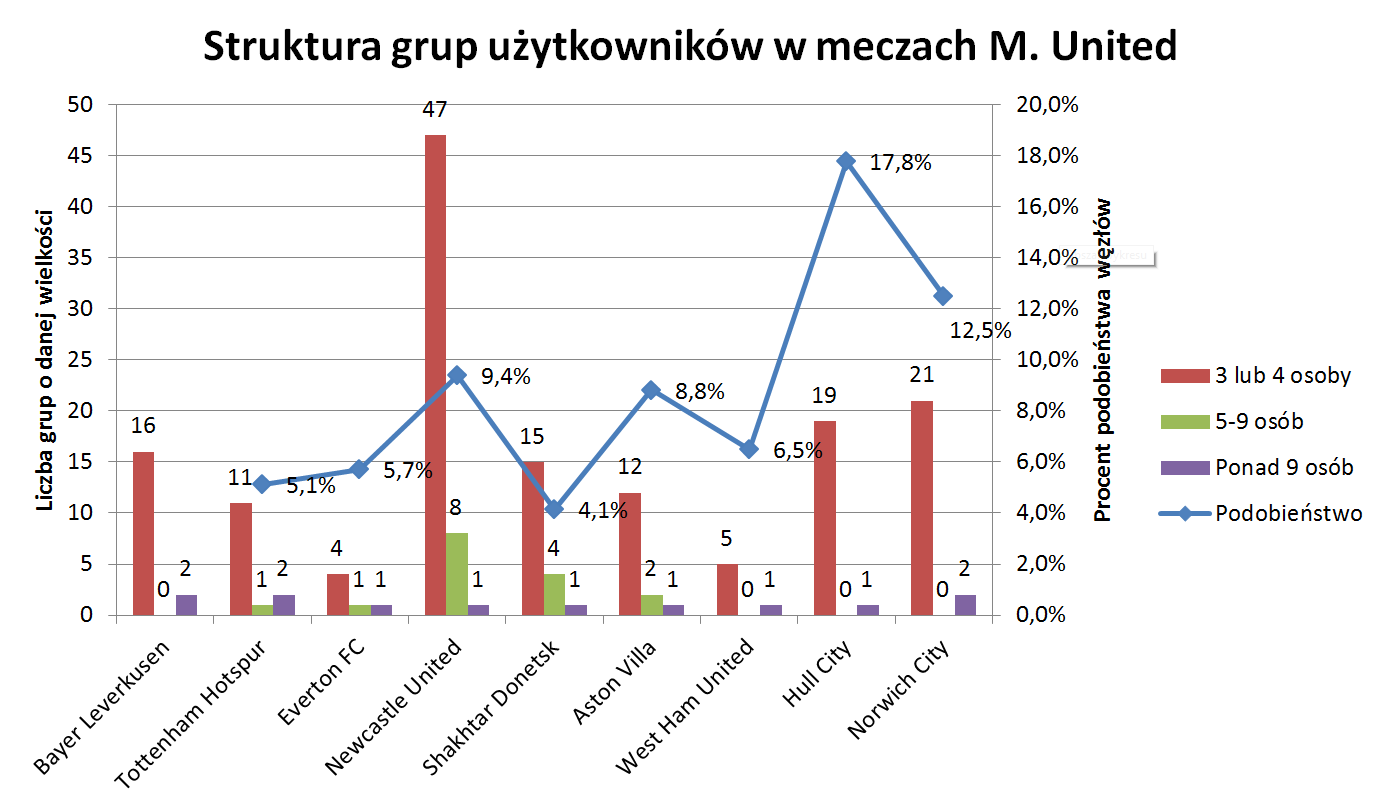
\includegraphics[width=160mm]{img/grupy-munited-nums.png}
\caption{Struktura grup użytkowników w meczach Manchesteru United}
\label{image:grupy-munited}
\end{figure}


\clearpage
\subsubsection{Obserwacje i wnioski}
Z analizy wykresów można zaobserwować, że w każdym spotkaniu najliczniejsze
są małe grupy -- 3 lub 4 osobowe. Liczba tych grup dodatkowo rośnie, gdy
mecz odbywa się z ciekawym przeciwnikiem. Na przykład zauważyć można, że
w meczach Arsenalu bardzo dużą liczbę grup wygenerowały spotkania
z Manchesterm Citym i Chelsea Londyn, a w meczach Manchestery United
skok liczby grup miał miejsce w meczu z Newcastle United.
Grupy liczniejsze jeśli chodzi o wielkość tworzyły się już zdecydowanie rzadziej.
I podobnie jak poprzednio ich większa liczbę również można zaobserwować
w ciekawszych spotkaniach.

Jeśli zaś chodzi o podobieństwo w kolejnych meczach to mamy tutaj do czynienia
z ciekawą, aczkolwiek zrozumiała sytuacją. Otóż im ciekawszy przeciwnik,
tym podobieństwo zbioru użytkowników w kolejnym meczu mniejsze.
Gdy drużyna -- w przypadku Arsenalu --  gra najpierw z Chelsea a później z 
West Ham United, to podobieństwo wynosi 3.7\%, a gdy najpierw gra z 
West Ham United -- w przypadku Manchesteru Untied -- a potem z Hull City
to podobieństwo między tymi meczami sięga 17.8\%.

Widać więc pewną charakterystyczną zależność. Gdy drużyna gra mecze z popularnymi
drużynami, wówczas liczba osób biorących na Twitterze udział w danym wydarzeniu
piłkarskim jest duża. Spotkanie takie absorbuje większą publikę. Stąd
większe słupki grup w popularnych meczach. Gdy jednak przeciwnik jest już nieco
mniej ciekawy, wówczas również zainteresowanie na Twitterze takim meczem spada.
Z tych prawidłowości wynika również dlaczego osiągany był taki, a nie inny
wynik podobieństwa. Otóż gdy zespół gra mecz to zawsze
wśród tweetujących na jego temat jest stała grupa fanów, która w spotkaniach
ze słabymi rywalami jest łatwiej dostrzegalna -- stanowi większy odsetek
wszystkich użytkowników Twittera. Gdy natomiast mecz jest interesujący
dla większej liczby odbiorców -- wówczas ta stała grupa fanów jest trudniej
dostrzegalna i odsetek podobieństwa drastycznie spada.
Mecze z ciekawymi rywalami przyciągają więc do siebie osoby okazjonalnie zainteresowane
danym temat -- te osoby następnym razem nie będą komentować meczu tej drużyny,
gdy ta będzie rozgrywać spotkanie z mało ciekawym rywalem. 
Wówczas jednak łatwiej będzie dostrzec tę grupę, która stanowi trzon zainteresowanych
daną drużyną i która jest jej stałym fanem.


% Podobieństwo węzłów między meczami 
% Podobieństwo grafów między meczami 
% Między mało popularnymi spotkaniami wysoki stopień podobieństwa
% +Sentyment a wielkość grupy











%%%%%%%%%%%%%%%%%%%%%%%%%%%%%%%%%%%%%%%%%%%%%%%%%%%%%%%%%% ANALIZA GEOGRAFICZNA

\section{Analiza geolokacji}
\label{section:analizageograficzna}

W moich badaniach skupiłem się także nad analizą użytkowników w oparciu 
o geolokalizację. Tak jak wspomniałem wcześniej, niewielka część wpisów
zawierała informacje o tym, z którego miejsca została wysłana.
Przy ich pomocy możliwe było dokonanie analizy danych związanych z położeniem
geograficznym.

\subsection{Odległość między użytkownikami a częstość kontaktów}
\label{subsection:odlegloscmiedzyuzytkownikami}
Zbadana została zależność pomiędzy tym jak często użytkownicy się ze sobą
komunikują, a tym w jakiej odległości fizycznej od siebie się znajdują (zgodnie
z opisem w sekcji \ref{subsubsection:zmierzenieodleglosci}). Wyniki przedstawia
poniższy wykres \ref{image:relacje-a-odleglosc}.

\begin{figure}[ht!]
\centering
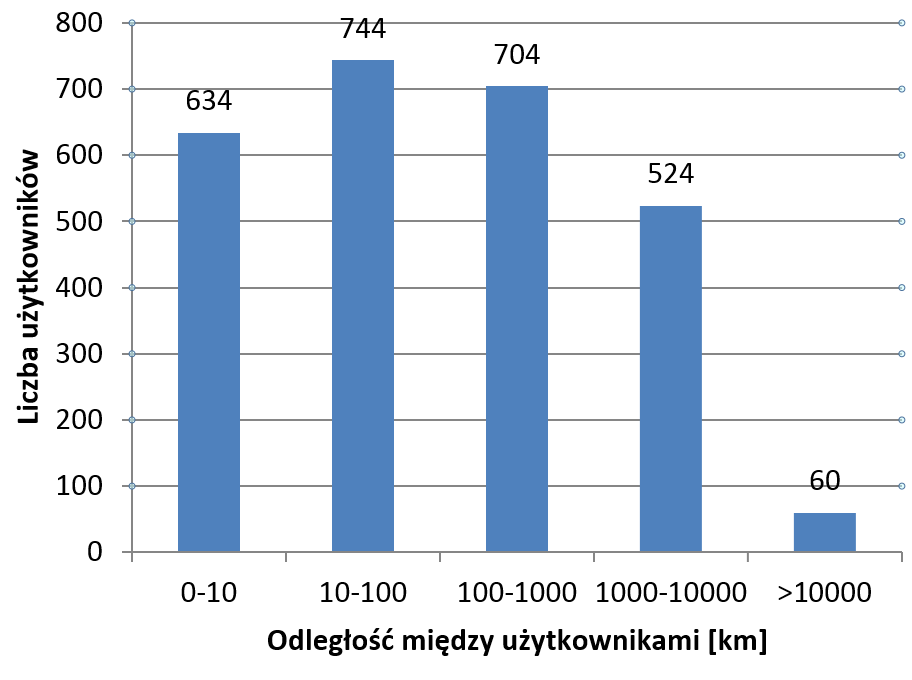
\includegraphics[width=140mm]{img/relacje-a-odleglosc.png}
\caption{Odległość między użytkownikami a częstość kontaktów}
\label{image:relacje-a-odleglosc}
\end{figure}

\subsubsection{Obserwacje i wnioski}
Każda kolejna kolumna na powyższym wykresie pokrywa obszar o dziesięciokrotnie 
większym promieniu. Oznacza to, że pole powierzchni, którego dotyczą rośnie
eksponencjalnie. Pomimo tego, liczba użytkowników, którzy wchodzili ze sobą
w interakcje jest za każdym razem tego samego rzędu.

Oznacza to więc, że im bliżej siebie byli użytkownicy fizycznie, tym częściej
odpowiadali na swoje wpisy. Gdy znajdowali się w odległości maksymalnie
10 kilometrów to do wymiany wpisów dochodziło tak samo
często, gdy byli od siebie oddaleni od 10 do 100 km, czy nawet od 100 do 1000 km.

Wniosek jest więc taki, iż pomimo tego, że internet nazywany jest globalną wioską
łączącą ludzi z całego świata, to użytkownicy komunikują się i tak z najbliższymi
sobie. Może to wynikać z kilku rzeczy. Na przykład osoby z Manchesteru 
prawdopodobnie będą kibicami drużyny United lub City i większe jest prawdopodobieństwo,
że będą komunikać się między sobą niż między osobami z innego miasta czy kraju.
Innym powodem takiego stanu rzeczy może być również bariera językowa.
Im dalej od danego kraju, tym mniej osób będzie w stanie posługiwać się językiem
tam panującym. Dodatkowym ograniczeniem może być czas lokalny, czyli strefy czasowe.
Gdy w jednym punkcie jest dzień, w drugim może być środek nocy jednoznacznie 
utrudniający komunikację między osobami z większych odległości.  

%Odległość od stadionu zwolenników, przeciwników 
%Odległość od stadionu a sentyment
%Miejscowości a sentyment 
%Kraje, a sentyment


\clearpage
\subsection{Rozkład wpisów na mapie}
\label{subsection:rozkladnamapie}
% Mecz Chelsea - Southampton, 01.12.2013 17:10.
Zebrane Tweety posiadające geolokalizację można przedstawić na
mapie\footnote{Załączone wizualizacje zostały stworzone przy pomocy serwisu
CartoDB (www.cartodb.com)}.
Poniżej na trzech kolejnych rysunkach zaprezentowany został rozkład wpisów,
które wysłane zostały podczas meczu Chelsea F.C. z Southampton F.C.
(01.12.2013 r.). Najpierw zaprezentowane są wpisy w skali całej Ziemii
\ref{image:mapa-swiata}, następnie w skali Wielkiej Brytanii
\ref{image:mapa-uk}, a na końcu zawierająca obszar między Londynem a Southampton
\ref{image:mapa-uk-zoom}, czyli miastami obu klubów.

\begin{figure}[ht!]
\centering
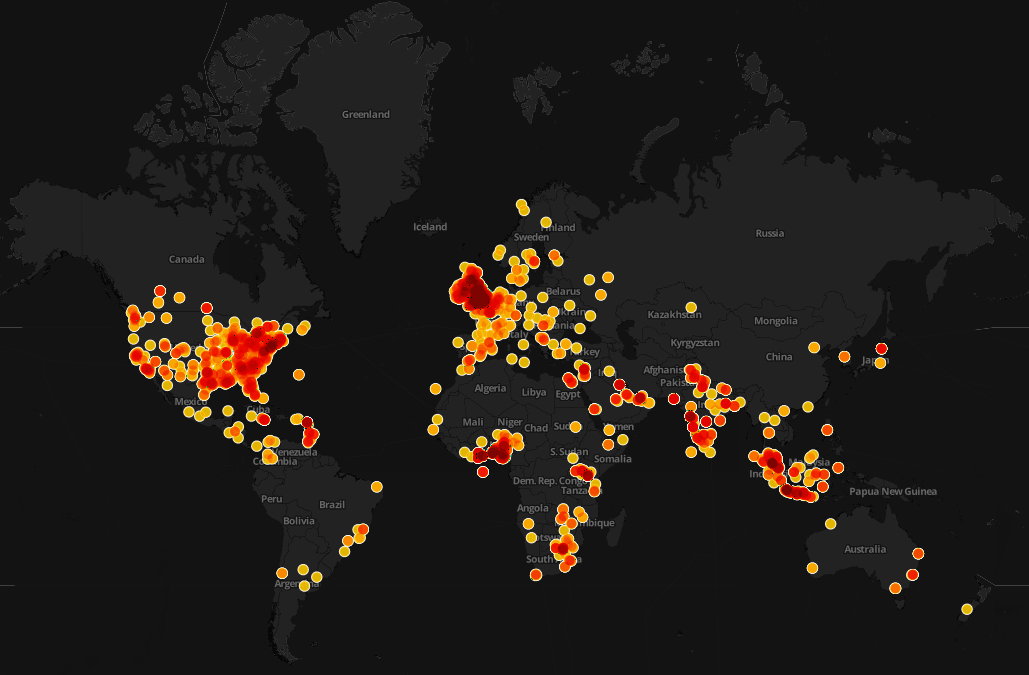
\includegraphics[width=140mm]{img/geo-chelsea-southampton.png}
\caption{Rozkład wpisów na mapie świata}
\label{image:mapa-swiata}
\end{figure}

Na powyższej wizualizacji wyróżnić można kilka krajów. Przede wszystkim na
pierwszym plan wyłania się Wielka Brytania -- z oczywistych względów, jako
miejsce, w którym odbywa się mecz oraz całe rozgrywki. Oprócz niej dużą liczbę
tweetów wysyła się z takich krajów jak między innymi:
Stany Zjednoczone (3 kraj pod względem liczby ludności na świecie, dominujący
język angielski), Indie (2 kraj pod względem ludności, j. angielski), Indonezja
(4 kraj pod względem ludności) a także państwa afrykańskie: Kenia i Uganda na
wschodze oraz Nigeria i Ghana na zachodzie. Należą one do najbardziej
zaludnionych krajów Czarnego Lądu i w każdym z nich język angielskim jest
językiem urzędowym.
Na mapie nie ma wpisów z Chin (najludniejszego kraju świata), gdzie Twitter
został zablokowany w 2009
roku\footnote{http://www.theguardian.com/technology/2009/jun/02/twitter-china}
oraz Rosji, w której popularniejsze są rodzime serwisy społecznościowe.

W meczu wzięli udział między innymi zawodnicy z Nigerii (John Obi Mickel -- Chelsea FC)
oraz Ghany (Michael Essien -- Chelsea FC, Victor Wanyama -- Southampton FC),
co zapewne wzmogło aktywność internautów z tych regionów.


\begin{figure}[ht!]
\centering
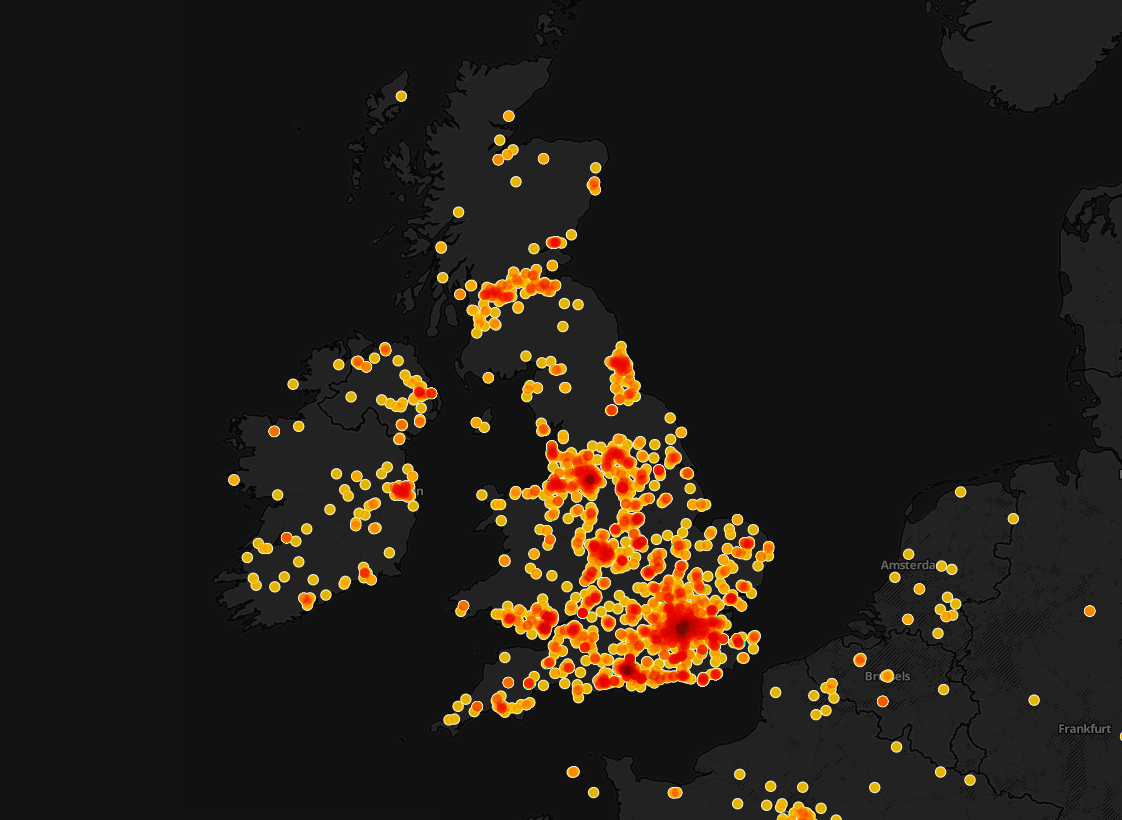
\includegraphics[width=140mm]{img/geo-uk-chelsea-southampton.png}
\caption{Rozkład wpisów w Wielkiej Brytani}
\label{image:mapa-uk}
\end{figure}

\begin{figure}[ht!]
\centering
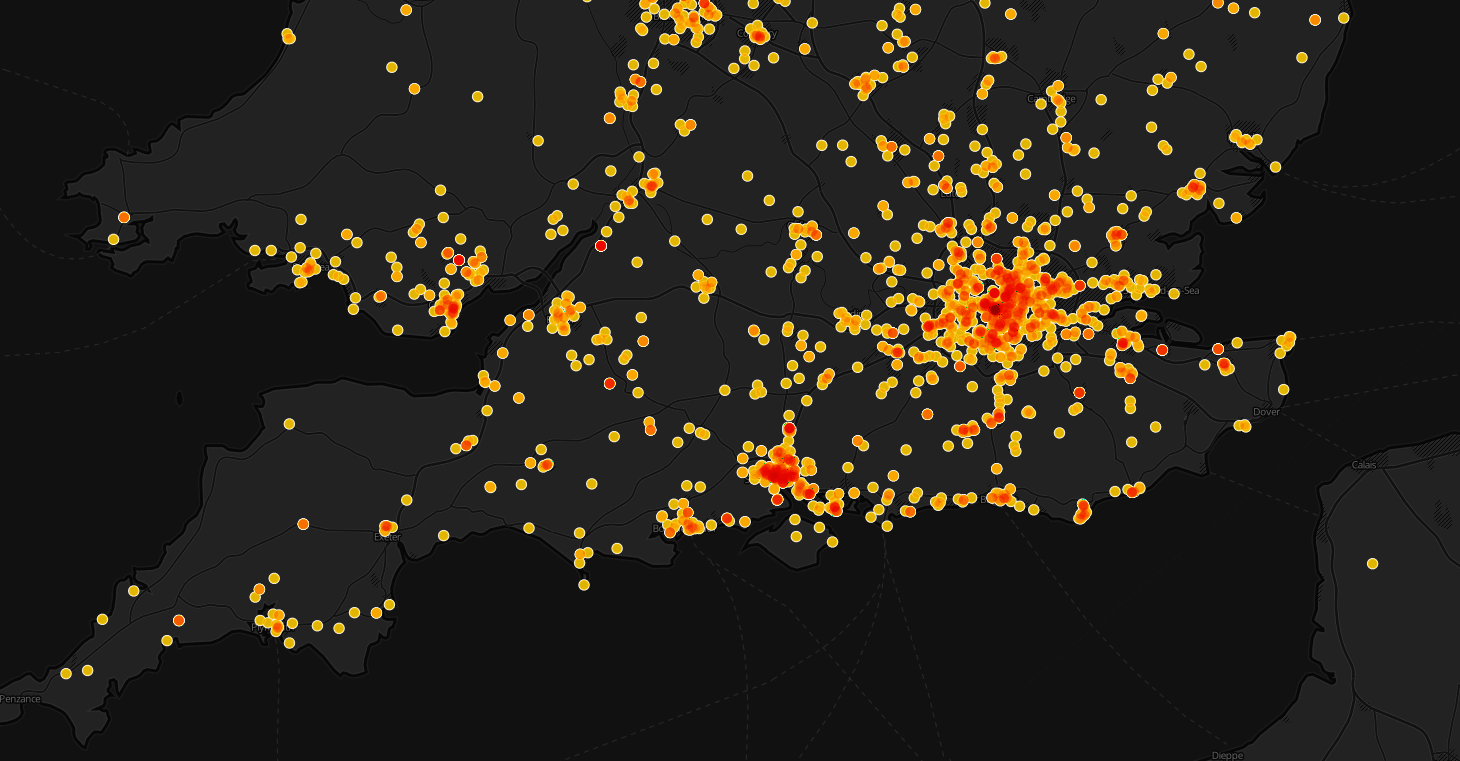
\includegraphics[width=140mm]{img/geo-uk-zoom-chelsea-southampton.png}
\caption{Rozkład wpisów wokół miast zespołów biorących udział w meczu}
\label{image:mapa-uk-zoom}
\end{figure}

Oceniając rozkład wpisów w Wielkiej Brytanii zauważymy dużą ich koncetrację wokół
Londynu -- największego miasta Zjednoczonego Królestwa (algomeracja Londynu to
ponad 13 milionów 
ludzi\footnote{2012 rok. Źródło: Eurostat (http://appsso.eurostat.ec.europa.eu/nui/show.do?dataset=met\_pjanaggr3\&lang=en)}).
Gdy zbliżymy mapę do obszaru Southampton i Londynu to za pomocą analizy rozkładu
wpisów na mapie bez problemu zlokalizujemy położenie tych miast.
Właśnie w nich znajduje się najwięcej ich kibiców generujących
największą liczbę wpisów.

Widać więc, że dane wydarzenie angażuje przede wszystkim osoby, którym jest ono
bliskie. Zastosowanie geolokalizacji pozwala nam te miejsca odkryć. I tak jak w
przypadku meczu piłarskiego można takie miejsca określić de facto jeszcze przed
analizą, tak w innego rodzaju badaniach przy użyciu tej techniki możliwe może
być odkrycie miejsc, obszarów geograficznych, o których nie myślałoby się w
kontekście badanego tematu. Powyższe wizualizacje potwierdzają stosowność
zastosowania geolokacji i jej skuteczności w różnego rodzaju badaniach
społecznych.

\subsection{Odległość od stadionu}
\label{subsection:odlegloscodstadionu}
Dane zawierające geolokalizację pozwalają wykonać szereg ciekawych eksperymentów.
Kolejnym z nich było zbadanie odległości kibiców od stadionu w zależności
od tego, czy drużyna grała mecz u siebie czy na wyjeździe. Dodatkowo
kibiców tych (dzięki analizie sentymentu) można było podzielić na zwolenników
i przeciwników. Takie badanie zostało przeprowadzone dla wszystkich meczów
Arsenalu Londyn a wyniki zaprezentowane są na rysunkach 
\ref{image:odleglosc-od-stadionu-gospodarz} i \ref{image:odleglosc-od-stadionu-gosc}.
Eksperyment ten został przeprowadzony zgodnie z opisem w sekcji
\ref{subsubsection:badanieodleglosciodstadionu}.

\begin{figure}[ht!]
\centering
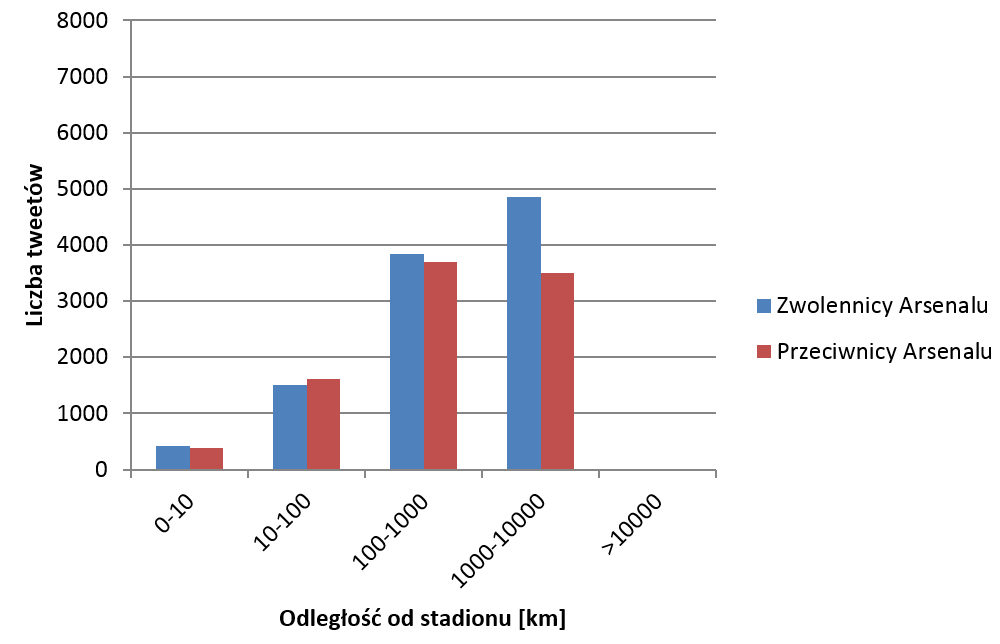
\includegraphics[width=140mm]{img/odleglosc-od-stadionu-home.PNG}
\caption{Odległość od stadionu w meczach Arsenalu u siebie}
\label{image:odleglosc-od-stadionu-gospodarz}
\end{figure}

\clearpage

\begin{figure}[ht!]
\centering
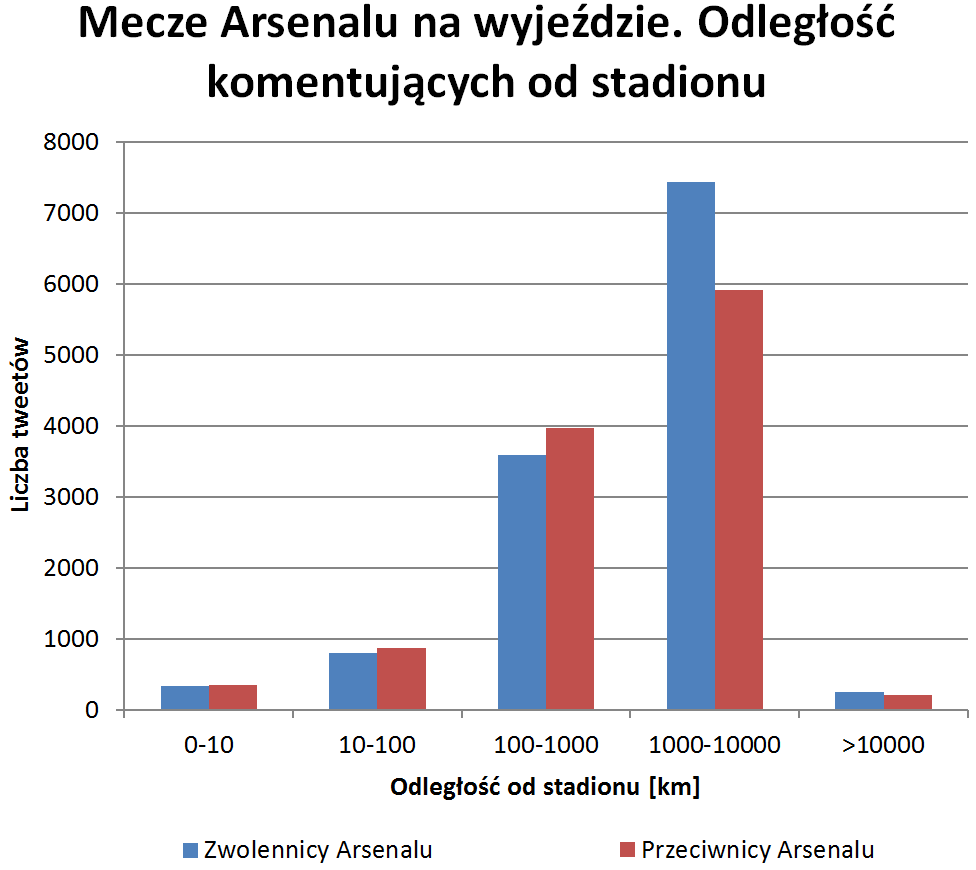
\includegraphics[width=140mm]{img//odleglosc-od-stadionu-away.png}
\caption{Odległość od stadionu w meczach Arsenalu na wyjeździe}
\label{image:odleglosc-od-stadionu-gosc}
\end{figure}

\subsubsection{Obserwacje i wnioski}
To co możemy na nich zaobserwować to fakt, że gdy Arsenal rozgrywa spotkanie na własnym
stadionie, wówczas liczba wpisów zwolenników przeważa wpisy przeciwników.
Zwłaszcza w odległości 0-10 i 10-100 kilometrów od stadionu.
Gdy natomiast mecz odbywa się na wyjeździe, wówczas lekko przeważające
są wpisy, których autorami są przeciwnicy Arsenalu.
W przypadku kiedy spojrzymy na kolumnę z wpisami wysyłanymi z odległości
1 - 10 tysięcy kilometrów od stadionu wtedy w obu przypadkach
więcej wpisów wysyłanych jest przez zwolenników londyńskiego klubu.

Widać więc, że spora część kibiców Arsenalu zapewne komentuje z Londynu
i nie przemieszcza się za swoją drużyną na każdy mecz. Wówczas, gdy klub rozgrywa
spotkanie na wyjeździe bliżej stadionu są kibice drużyny przeciwnej,
którzy tworzą wpisy odznaczające się raczej niechęcią do Arsenalu. 
Jeśli natomiast
chodzi o kibiców z dalszych zakątków świata to można stwierdzić, że
jeśli interesują się oni tą drużyną, to raczej nastawieni są do niej pozytywnie
i łatwiej jest o sympatyków niż antyfanów.


\clearpage
\subsection{Rozkład wpisów z geolokacją w trakcie meczu}
\label{subsection:geowpisy}
Pośród wszystkich zebranych tweetów tylko 3.06\% z nich zawierało informacje o
geolokacji. Poniżej na podstawie meczu Chelsea F.C. z Southampton F.C.
(01.12.2013 r.) zaprezentowano porównanie
(rys. \ref{image:wpisy-odsetek-geotagged}) liczby wpisów z geolokacją do
wszystkich wpisów.

\begin{figure}[ht!]
\centering
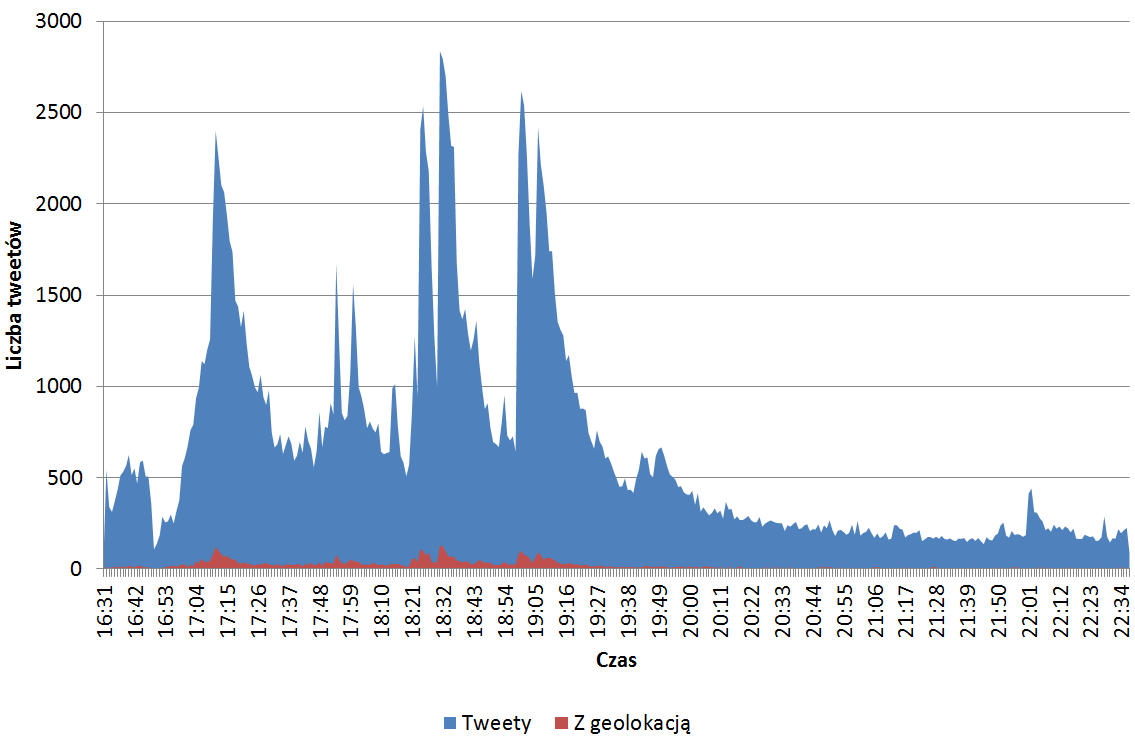
\includegraphics[width=140mm]{img/tweet-geo-w-meczu.PNG}
\caption{Rozkład wpisów z geolokacją w trakcie meczu}
\label{image:wpisy-odsetek-geotagged}
\end{figure}

\subsubsection{Obserwacje i wnioski}
Wykres jednoznacznie obrazuje o jakiej różnicy jest mowa. Nieco ponad 3\% 
wpisów z geolokacją to bardzo niewiele. Widać, że liczba takich tweetów
rośnie w tych samych momentach, gdy rośnie ogólna liczba wpisów.
Niestety (z punktu widzenia badań) geotagowanie wpisów
nie jest jeszcze czymś powszechnym i zapewne musi minąć trochę czasu,
by użytkownicy serwisów społecznościowych chętniej dzielili się miejscem,
w którym się znajdują.

\begin{comment}
\clearpage
\subsection{*Sentyment a położenie geograficzne}
Dzięki zastosowaniu georeversingu przy pomocy Open Street Map,
możliwe było odczytanie ze współrzędnych tweetów zawierających geolokalizację
szczegółów dotyczących danego miejsca.
Tym sposobem, do każdego wpisu dołączone zostały informacje o kraju,
hrabstwie/powiacie oraz mieście, z którego został on wysłany. W połączeniu z
analizą sentymentu zaprezentować można nastroje jakie pojawiają się
w różnych miejscach. Poniżej przedstawiam wykresy pokazujące wartość
sentymentu w różnych obszarach geograficznych, które zostały zaobserwowane
podczas meczu Chelsea F.C. z Liverpool F.C. (29.12.2013 r.) zakończonego
wynikiem 2-1. Są to rysunki z sentymentem w krajach \ref{image:sentyment-kraje},
powiatach/hrabstwach (ang. county) \ref{image:sentyment-hrabstwa}
oraz miastach \ref{image:sentyment-miasta}.

\begin{figure}[ht!] 
\centering
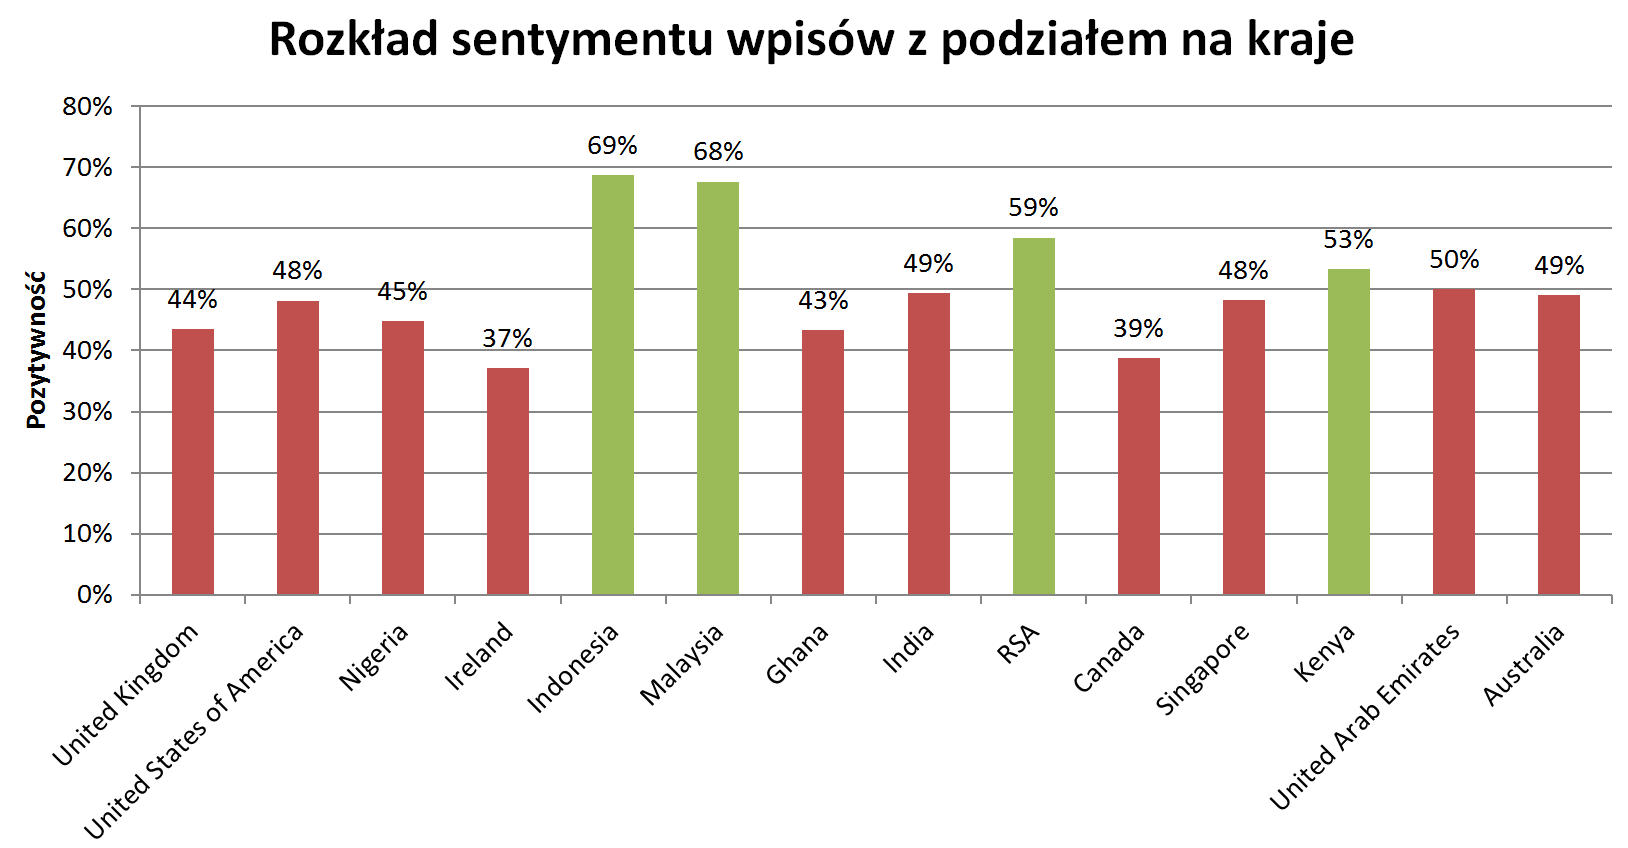
\includegraphics[width=140mm]{img/sentyment-kraje.PNG}
\caption{Sentyment wpisów z podziałem na kraje}
\label{image:sentyment-kraje}
\end{figure}

\begin{figure}[ht!]
\centering
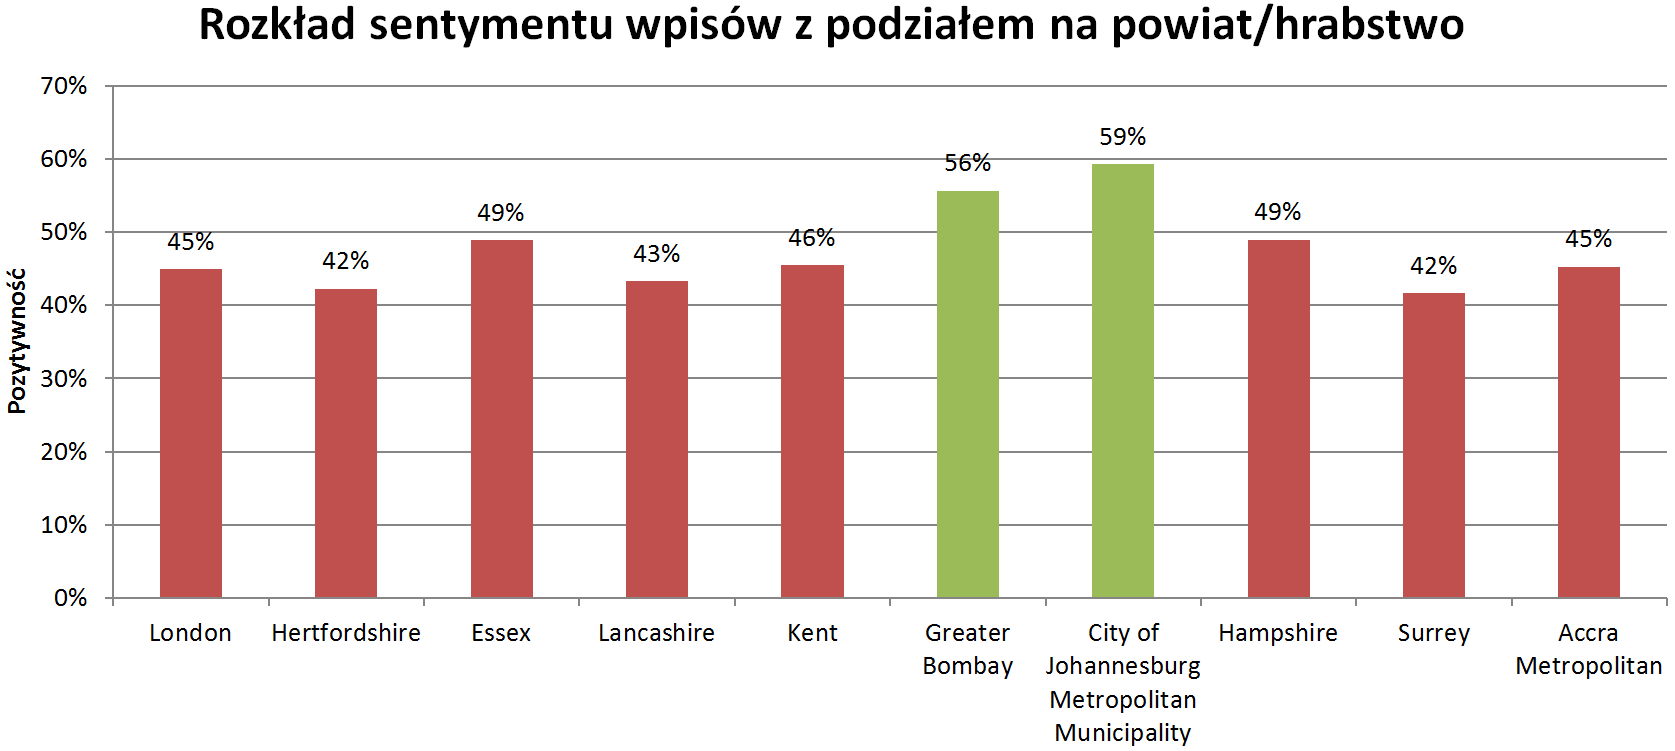
\includegraphics[width=140mm]{img/sentyment-powiaty.PNG}
\caption{Sentyment wpisów z podziałem na powiat/hrabstwo}
\label{image:sentyment-hrabstwa}
\end{figure}

\clearpage

\begin{figure}[ht!]
\centering
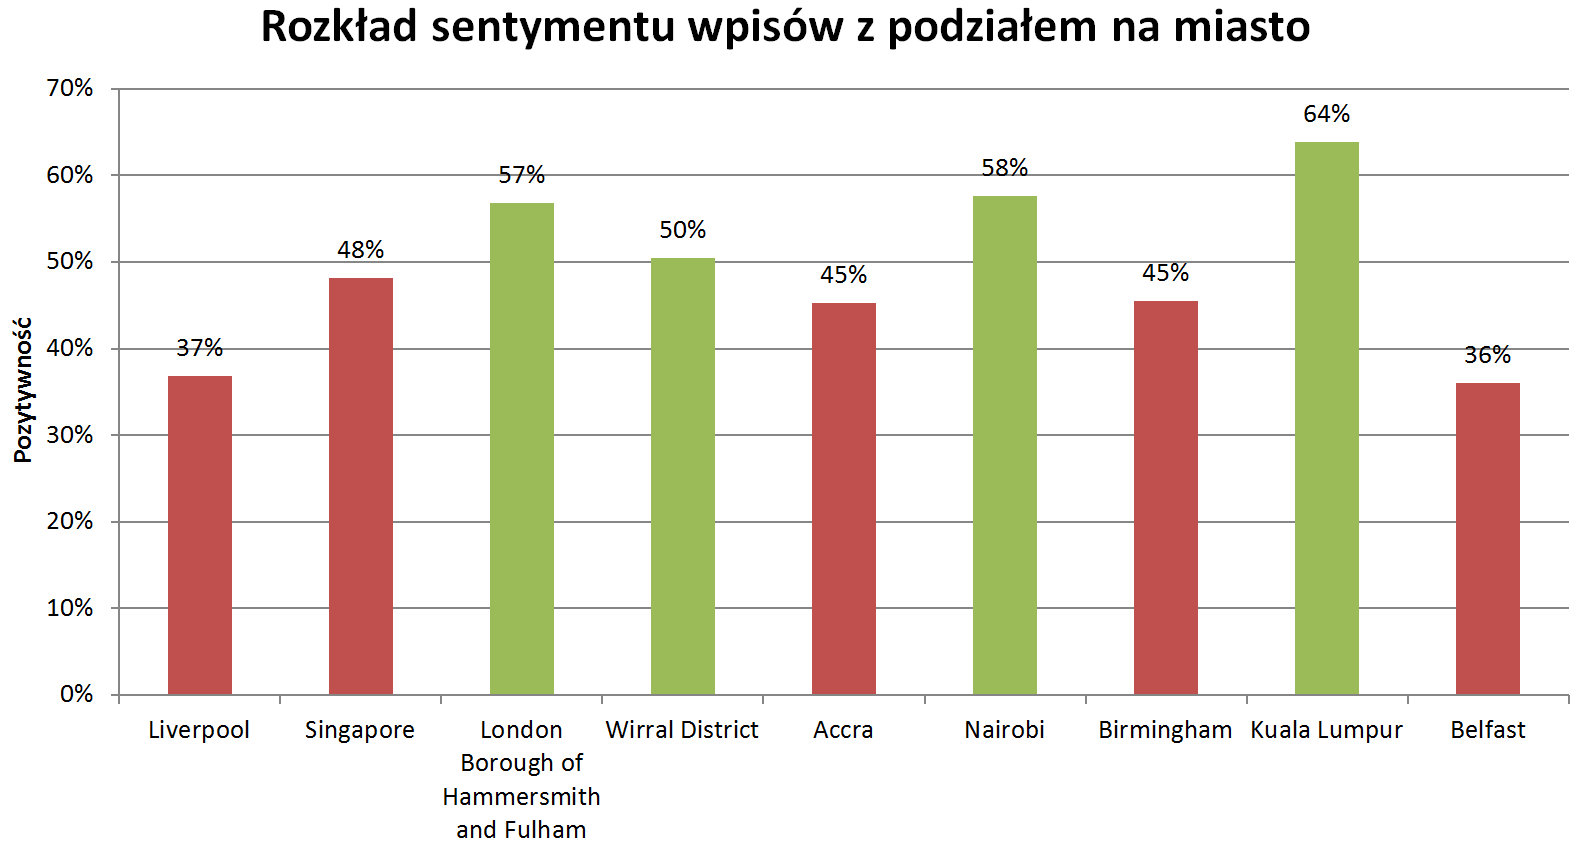
\includegraphics[width=140mm]{img/sentyment-miasto.PNG}
\caption{Sentyment wpisów z podziałem na miasta}
\label{image:sentyment-miasta}
\end{figure}

\subsubsection{Obserwacje i wnioski}
\end{comment}
















%%%%%%%%%%%%%%%%%%%%%%%%%%%%%%%%%%%%%%%%%%%%%%%%%%%%%%%%%% PODSUMOWANIE
\section{Podsumowanie eksperymentów}
Zaprezentowane powyżej eksperyment potwierdziły, że zastosowane przeze mnie
podejście do analizy dużej sieci społecznej z wykorzystaniem analizy sentymentu
i geolokacji powiodło się. Przedstawiony w rozdziale
\ref{section:analizasentymentu} okazał się skutecznym narzędziem pokazującym
zmieniające się nastroje wśród kibiców, a także pomógł zbadać sposoby interakcji
między nimi z podziałem na zwolenników i przeciwników. Geolokacja, chociaż
jeszcze niezbyt popularna, pokrywa się z tym, czego można się spodziewać. 
Najwięcej wpisów pochodzi z miejsc, w których faktycznie jest zainteresowanie
danym tematem. Okazało się, że kibice najchętniej komentujące mecze z
największymi rywalami, a podobieństwo zbioru użytkowników między kolejnymi
spotkaniami jest tym większe, im mniej popularny jest mecz -- potwierdzając tym
samym, że to najzagorzalsi fani są ze swoim klubem niezależnie od sytuacji.

Przeprowadzone eksperymenty udowodniły, że można wykorzystać nowoczesne techniki
komputerowe do badania dużych sieci społecznych wzbogacając je o analizę
sentymentu i geolokację, które służą do lepszego zrozumienia badanych
społeczności.


